\chapter{Functions}
\label{sec:functions}

\epigraph{The art of doing mathematics is finding that special case that contains all the germs of generality. }{\textit{David Hilbert}}

\section{What is a function}
The concept of a function is essential to understand not just calculus but also computer programming. We can think of a function as being a black box that takes in information, potentially changes it in some way, and then outputs information.\\

\begin{figure}[ht]
    \centering
    %\pdftooltip{
    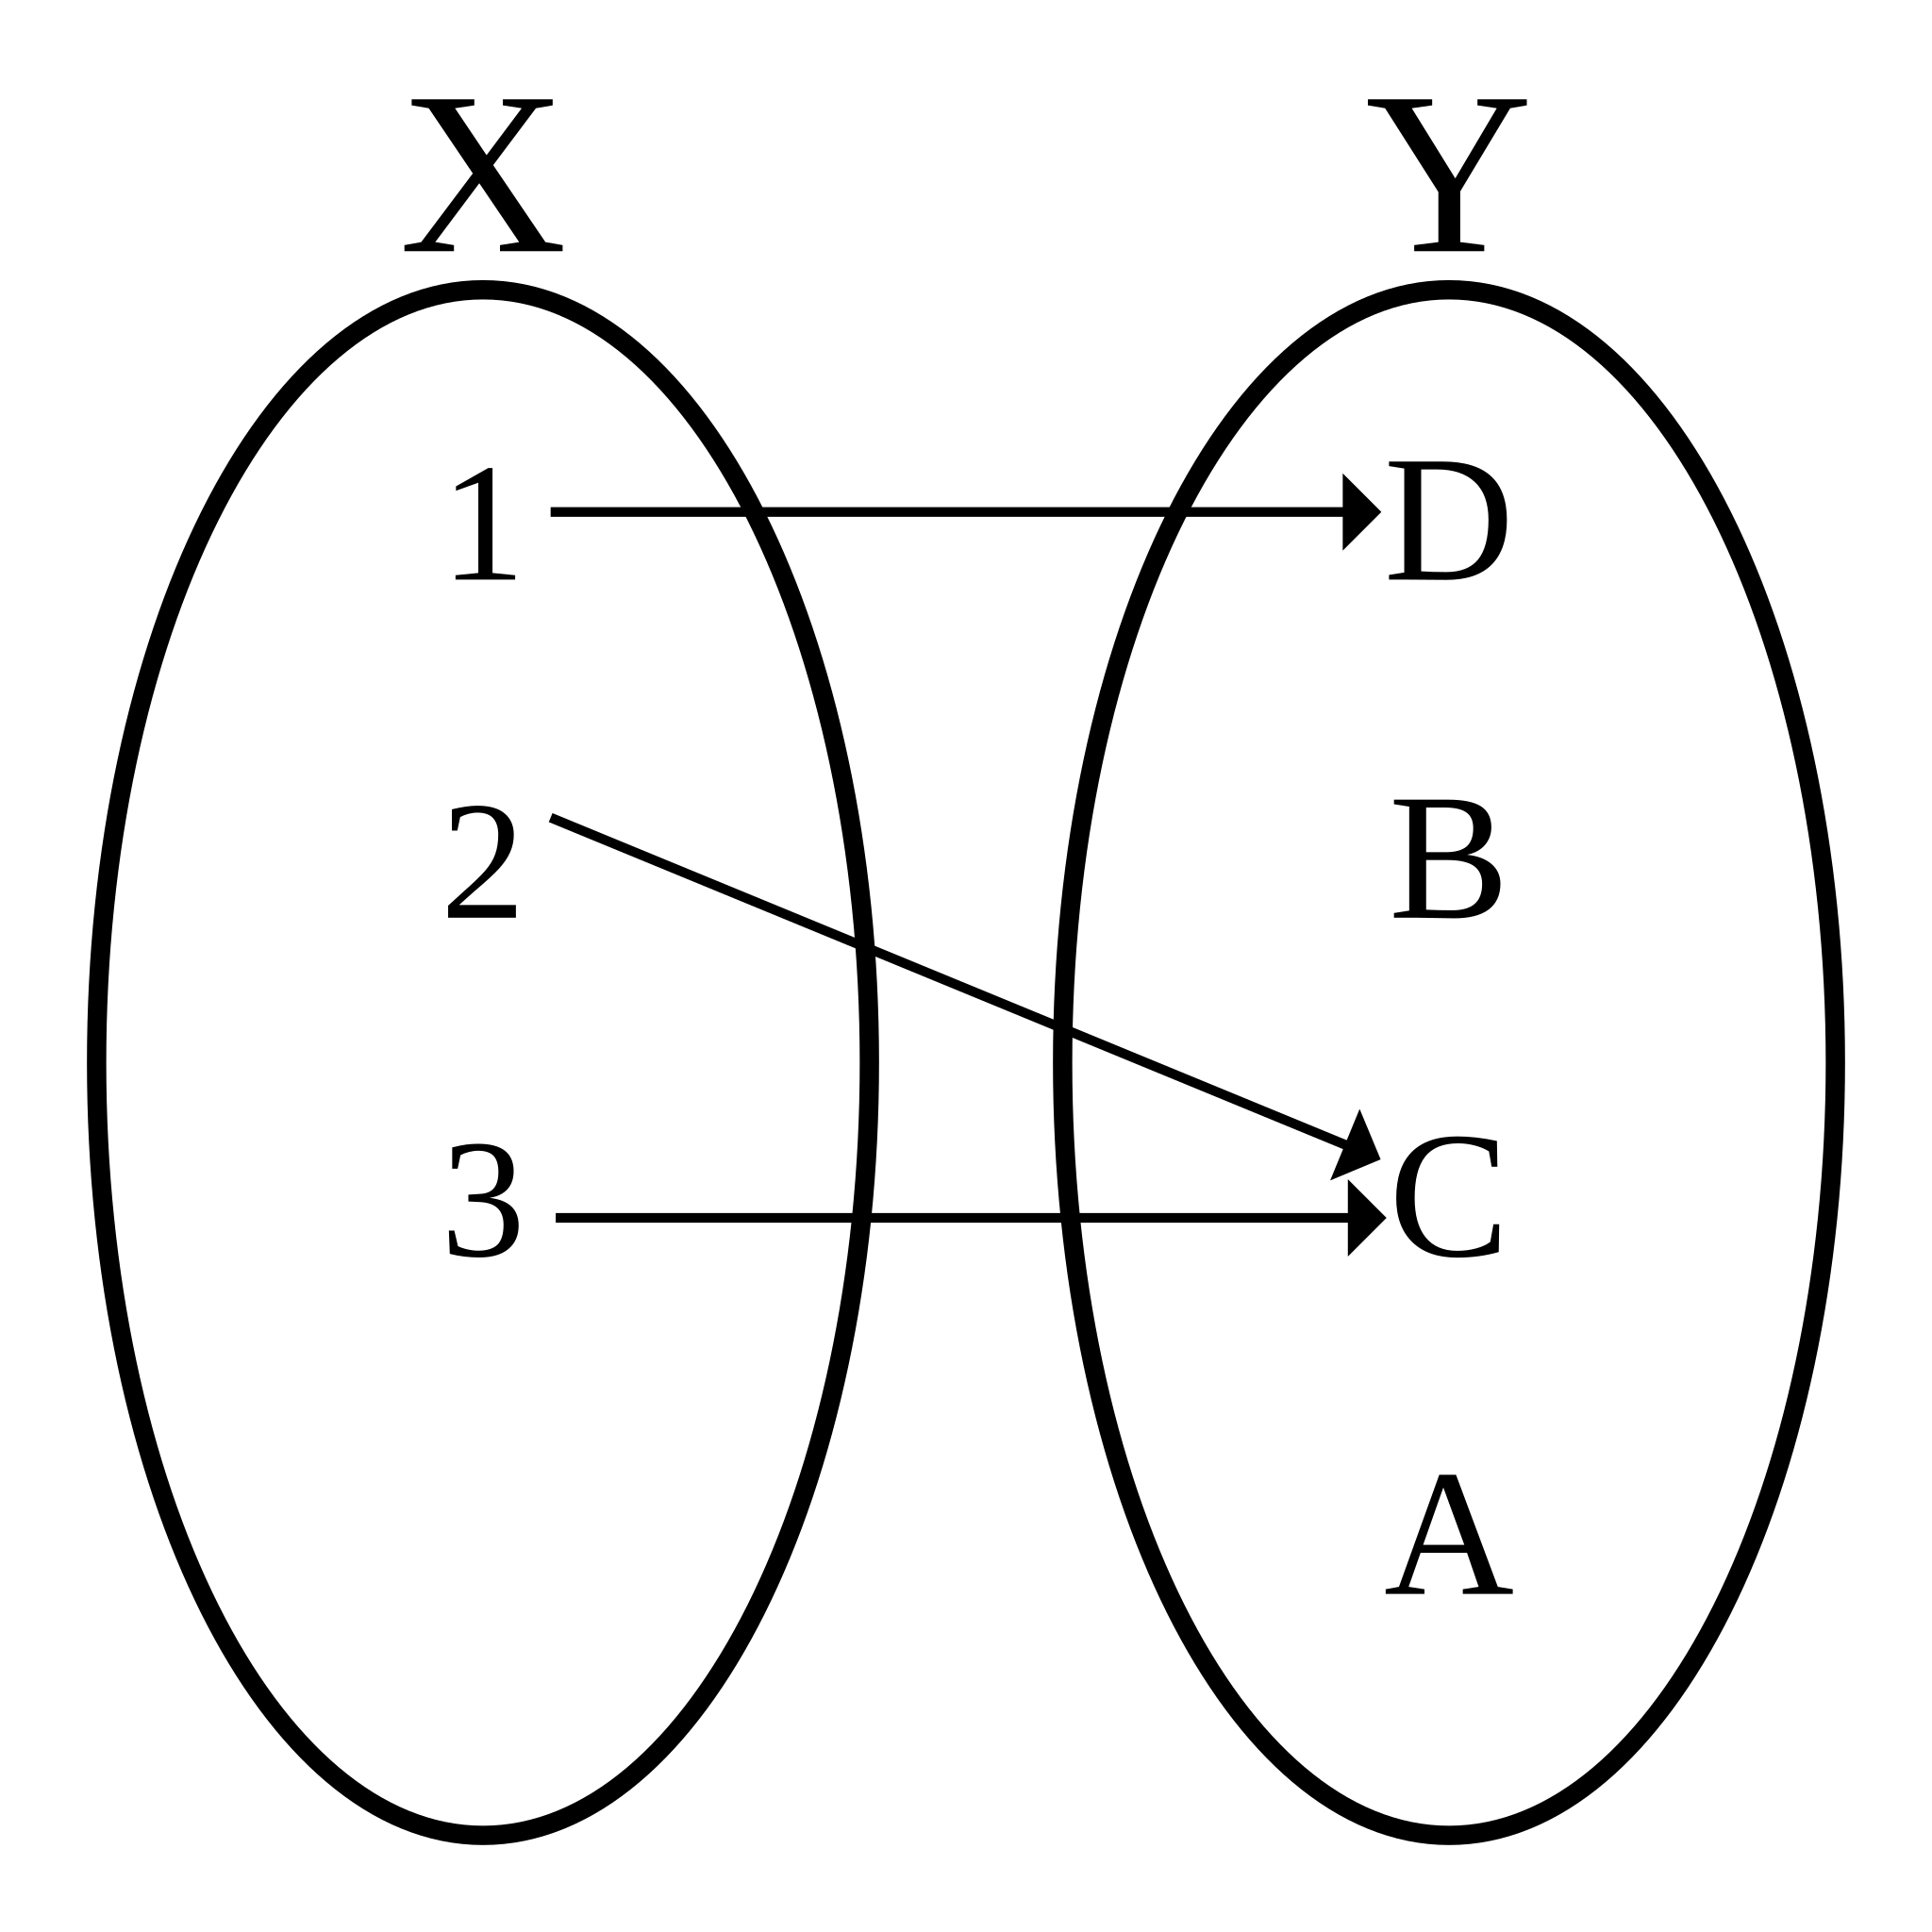
\includegraphics[width=0.3\textwidth, alt ={A schematic of how a function behaves produced by Bin Im Garten for Wikimedia Commons.}]{figures/Injection_keine_Injektion_2a.png}
    %}{A schematic of how a function behaves produced by \href{Bin Im Garten} for Wikimedia Commons. }
    \caption{A schematic of how a function behaves, it maps objects $1,2,3,\dots$ in the \gls{set} $X$ to objects $A,B,C,D,\dots$ in the set $Y$. This image was produced by \href{https://commons.wikimedia.org/wiki/File:Injection\_keine\_Injektion\_2a.svg}{Bin Im Garten} for Wikimedia Commons.}
\label{fig: function schematic}
\end{figure}

Being more precise, a function is a map between two spaces, the domain, and the codomain. e.g.
\begin{equation*}
f:X\to Y
\end{equation*}
and it sends a point $x\in X$ to a point $f(x)=y\in Y$.  Functions have the property that they map a point $x\in X$ to a single point $y\in Y$,for example:
\begin{equation*}
y=f(x)=x^{2}+1,
\end{equation*}
is a function since every value of $x$ gives a single value of $y$. However, 
\begin{equation*}
y^{2}=x+1,
\end{equation*}
is not a function since every $x$ corresponds to two values of $y$, e.g. if $x=3$ then $y^{2}=3+1=4$ and $y$ can be both $2$ and $-2$.\\

Note that when we write $f(x)$ we are not saying $f$ times $x$, but mean that $f$ is a function of $x$, e.g. $f$ takes in a value of $x$ and returns a number $y=f(x)$.\\

Throughout this module we will meet several different types of functions so you will need to get familiar with this notation and understand how to evaluate functions. There will be some questions in the tutorial sheet to help you practice this.\\

A key property of a function is its \textbf{\gls{roots}} or zeros, these are the values of $x$ such that $f(x)=0$. For linear functions finding the roots is just a matter of rearranging the equation, sometimes referred to as changing the subject. In this module I am assuming that you have some familiarity with this, if not take a look at the background material in \cref{sec:background} or ask me to point you towards more resources. There will also be some revision questions on this topic in the first couple of weeks tutorials.

\begin{ex} Find all the roots of $f(x)=9x^{3}-18x^{2}+6x$.\\

Remember the roots are where $f(x)=0$ so we are solving $9x^{3}-18x^{2}+6x=0$. First notice that there is a common factor of $3x$ in all of the terms so we can factor that out and get
\begin{equation*}
0=9x^{3}-18x^{2}+6x=3x\left(3x^{2}-6x+2\right).
\end{equation*}
This means that either $x$ is zero or the quadratic expression in brackets, $3x^{2}-6x+2$, is zero. This means that $x=0$ is a root of the equation, and there will be two more that we find by solving the quadratic. This can be done by using the quadratic formula:
\begin{align*}
x&=\frac{6\pm\sqrt{(-6)^{2}-4(3)(2)}}{2(3)}\\
&=\frac{6\pm\sqrt{12}}{6}\\
&=1\pm\frac{\sqrt{3}}{3}\\
&=1\pm\frac{1}{\sqrt{3}}.
\end{align*}

So the three roots of $f(x)$ are
\begin{equation*}
x=0,\quad x=1+\frac{\sqrt{3}}{3},\quad x=1-\frac{\sqrt{3}}{3}.
\end{equation*}

\end{ex}

If you do not remember how to use the quadratic formula then I suggest that you look at the background material in \cref{sec:background}.\\

If this was a course for mathematicians this is where we would spend time talking about the domain and range of a function. How they are defined, and when we need to be careful to avoid dividing by zero. Here, we will not go through this, and I will just remind you that in your algebraic manipulations you should not divide by any quantity that is zero.\\

A simple, yet useful, class of functions are the rational functions. There are functions who are the ratio of two polynomials, e.g. 
\begin{equation*}
f(x)=\frac{4x+10}{x^{2}-2x-15}.
\end{equation*}

A useful way to understand a function is draw a graph. In a graph, the domain of the function $X$ is drawn horizontally and the codomain, $Y$, is drawn vertically, using \textbf{\gls{Cartesian} axes} $(x,y)$. The graph consists of the points $(x,y)$ with $y=f(x)$. In many books $x$ is called the independent variable and $y$ the dependent variable. In the tutorials we will discuss how to produce plots using a computer, either using \textbf{MATLAB}, \textbf{Python}, or \href{https://www.wolframalpha.com/}{\textbf{WolframAlpha}}. There are also online graphing programs like \href{https://www.desmos.com/}{\textbf{desmos}} and \href{https://www.geogebra.org/}{\textbf{GeoGebra}}. In these notes most of the graphs are produced using the Tikz package for \LaTeX{}, which is a typesetting and markup language\footnote{If you want to produce professional looking documents which include mathematical formulas then it is worth your time learning how to use \LaTeX{}.}.

\begin{ex}
Plot the graph of $f(x)=2x^{2}-1$.\\
\begin{figure}[htbp]
    \begin{center}
\ThisAltText{Graph of a quadratic.}
   % \pdftooltip{
    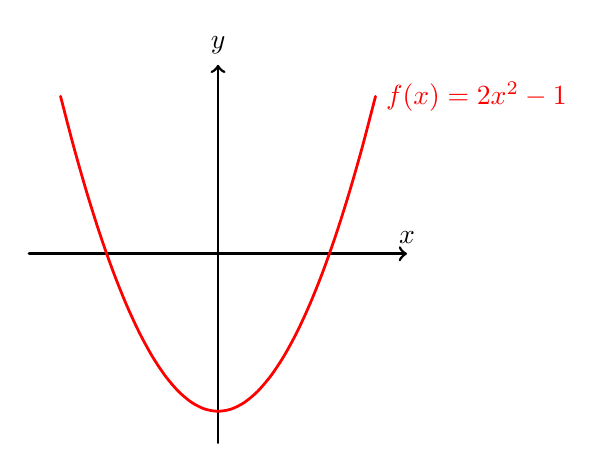
\begin{tikzpicture}[line width=1pt,line cap=round,line join=round,domain=-1:1, smooth,variable=\x,scale=2]
     \draw[->] (-1.2,0) -- (1.2,0) node[above] {$x$};
  \draw[->] (0,-1.2) -- (0,1.2) node[above] {$y$};
 \draw[color=red]   plot (\x,{2*\x*\x -1}) node[right] {$f(x)=2x^{2}-1$};
    \end{tikzpicture}
%    }{graph of a quadratic}
    \caption{The graph of the quadratic function  $f(x)=2x^{2}-1$ is a parabola which intersects the $y$-axis at $x=0$ and the $x$-axis at $x=\pm\frac{1}{\sqrt{2}}$.}
        \label{fig: quadratic function graph}
\end{center}
\end{figure}
\end{ex}
Note that the equation $y^{2}=x+1$ also defines a parabola, see \cref{fig: non equation}. However if we plot this function the curve is not the graph of a function. You should think about why this is.

\begin{figure}[ht]
    \centering
    %\pdftooltip{
    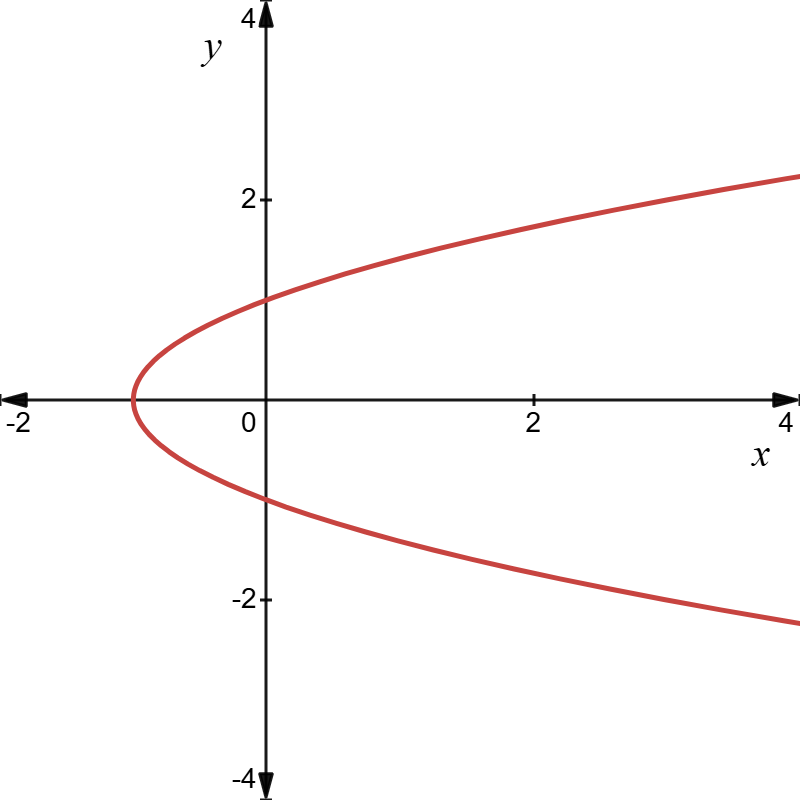
\includegraphics[width=0.4\textwidth, alt={An equation which does not give a graph.}]{figures/desmos-graph_non-function}
    %}{An equation which does not give a graph. }
    \caption{A plot of $y^{2}=x+1$, you should think about why this is not the graph of a function. }
\label{fig: non equation}
\end{figure}

\begin{ex}The function $f(x)=\sin(x)$ has the graph shown in \cref{fig: sine function graph}.\\
\begin{figure}[htbp]
    \centering
\ThisAltText{graph of sin(x).}
  %  \pdftooltip{
    \begin{tikzpicture}[line width=1pt,line cap=round,line join=round,domain=-6.282:6.282, smooth,variable=\x]
     \draw[->] (-6.282,0) -- (6.282,0)node[above] {$x$};
  \draw[->] (0,-1.2) -- (0,1.2) node[above] {$y$};
 \draw[color=CDred]   plot (\x,{sin(\x r)}) node[right] {$f(x)=\sin(x)$};
    \end{tikzpicture}
  %  }{graph of sin}
    \caption{The graph of the sine function  $f(x)=\sin(x)$.}
        \label{fig: sine function graph}
\end{figure}
\end{ex}

\begin{ex}
Consider the two functions $f(x)=3x-2$ and $g(x)=x/3 +2/3$. These satisfy the relationship
\begin{align*}
\left(f\circ g\right)(x)	&=f\left(g(x)\right)\\
				&=f\left(\frac{x}{3}+\frac{2}{3}\right)\\
				&=3\left(\frac{x}{3}+\frac{2}{3}\right)-2\\
				&=x+2-2=x
\end{align*}
and 
\begin{align*}
\left(g\circ f\right)(x)=x.
\end{align*}

When we have two functions whose composition leaves $x$ unchanged, we say that they are \textbf{\gls{inverse}} to each other, and $g$ is the inverse\footnote{Usually the inverse function is denoted as $f^{-1}$, though we need to be careful to understand that this does not mean $1/f$.} of $f$. As can be seen in Section 1.2 of \citep{calcI} we can understand this a meaning that if $f:x\mapsto y$ then $g:y\mapsto x$, e.g. $f(-1)=-5$ while $g(-5)=-1$.
\end{ex}

The concept of an inverse function makes intuitive sense. However, if we pretend to be mathematicians and treat this carefully we quickly encounter some problems. For example, what happens if we have a function which sends two different values of $x$ to the same value? Then we are unable to know which value we started with, so cannot build an inverse function. For example $f(x)=x^{2}$ sends both $x$ and $-x$ to $x^{2}$ so we cannot find an inverse that works everywhere, this is why when we firts meet the square root function you often see it as $\pm\sqrt{\phantom{+}}$.\\

Mathematicians fix this by introducing the notion of a \textbf{\gls{one-to-one}} function, sometimes called an \textbf{injective} function. A function is called one-to-one if no two values of $x$ produce the same value of $y$, so that
\begin{equation*}
f(x_{1})\neq f(x_{2}) \qquad \text{ for } x_{1}\neq x_{2}.
\end{equation*}

The advantage of one-to-one functions is that we can find inverses for them. If we have two one-to-one functions which satisfy 
\begin{equation*}
\left(f\circ g\right)(x)=x=\left(g\circ f\right)(x),
\end{equation*}
then $f$ and $g$ are inverses and we write $g(x)=f^{-1}(x)$.

\section{Trigonometric functions}
\label{sec: trig func}

Now that we have discussed functions and how to graph them, we can focus on some specific functions which it is very common to encounter.\\ 

From your previous maths experience you have probably come across \textbf{\gls{trigonometric}} (trig) functions in the context of triangles, where they are used to calculate lengths and angles. If you do not remember how this works then I suggest that you have a look at the Triganometry primer in \cref{sec:background} or check out some revision material available \href{https://corbettmaths.com/2013/03/30/trigonometry-introduction/}{here}. Another important thing to remember is that you should always work in radians rather than degrees when using trig functions. This is because radians are a more natural unit for angles and if we did not use them lots of formulas would need extra factors of $\uppi$ to be added for them to be valid. \\

\begin{figure}[ht]
    \centering
\ThisAltText{Converting from a circle to trig functions.}
  %  \pdftooltip{
    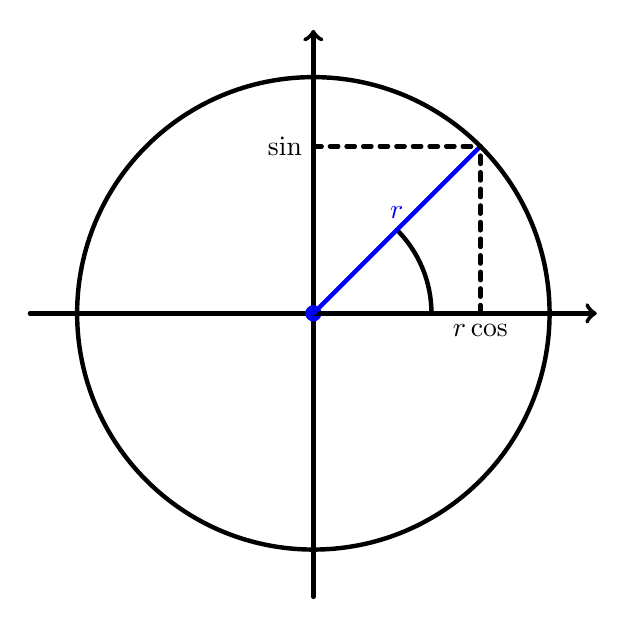
\begin{tikzpicture}[line width=1pt,line cap=round,line join=round, scale = 1.5]
   % \draw[step=1cm,gray,very thin] (3,-3) grid (3,3);
   \draw[->,ultra thick] (0,-2.4)--(0,2.4);
     \draw[->,ultra thick] (-2.4,0)--(2.4,0);
   \filldraw[color = blue, ultra thick](0,0) circle (0.05);
    \draw[ ultra thick](0,0) circle (2);
    \draw[ultra thick] (0,0) -- (2,0);
    \draw[ultra thick] (1,0) arc (0:45:1) node[anchor=north]{$\ut$};
     %\draw[ultra thick, color=red] (2,0) arc (0:45:2) node[anchor=north]{$s$};
     \draw[color = blue, ultra thick](0,0)--node[anchor=south]{$r$}(1.414,1.414) ;
     \draw[dashed, ultra thick] (0,1.414)node[left]{$\sin\ut$} --(1.414,1.414);
      \draw[dashed, ultra thick] (1.414,0) node[below]{$r\cos\ut$}--(1.414,1.414);
    \end{tikzpicture}
 %   }{Converting from a circle to trig functions}
    \caption{Trig functions and their relationship to a unit circle, this is true whatever the angle $\ut$ is, though we need to be careful about the signs of $x$ and $y$ }
        \label{fig:trig and circles}
\end{figure}


In the setting of triangles the angles are restricted to run between $0$ and $\uppi$ radians as for angles greater than this we would no longer have a triangle. However, the functions are valid for any real values of the argument, $x$. Typically we will be interested in angles within the range $[0,2\uppi)$, but need to remember that, as shown in \cref{fig: trig functions}, these functions are $2\uppi$ periodic. This means that
\begin{align*}
\sin(x+2\uppi)=\sin(x),\\
\cos(x+2\uppi)=\cos(x),\\
\tan(x+2\uppi)=\tan(x).
\end{align*}

We can think of these as functions from $[0,2\uppi)\to [-1,1]$ which reduce to the familar trig functions for angles between $0$ and $\uppi$.\\

\begin{figure}[ht]
    \centering
\ThisAltText{Graph of sin(x) and cos(x).}
   % \pdftooltip{
    \begin{tikzpicture}[line width=1pt,line cap=round,line join=round,domain=-6.28:6.28, smooth,variable=\x]
     \draw[->] (-7,0) -- (7,0) node[above] {$x$};
  \draw[->] (0,-1.3) -- (0,1.3);
 \draw[color=CDnavy]   plot[samples=300] (\x,{cos(\x r)}) node[right] {$\cos(x)$};
  \draw[color=CDgreen, dashed]   plot[samples=300] (\x,{sin(\x r)}) node[anchor = north west] {$\sin(x)$};
    \end{tikzpicture}
 %   }{plots of sin and cos }
    \caption{Plots of the trig functions $\sin(x)$ and $\cos(x)$ for $x$ between $-2\uppi$ and $2\uppi$.}
        \label{fig: trig functions}
\end{figure}


\begin{figure}[ht]
    \centering
  %  \pdftooltip{
  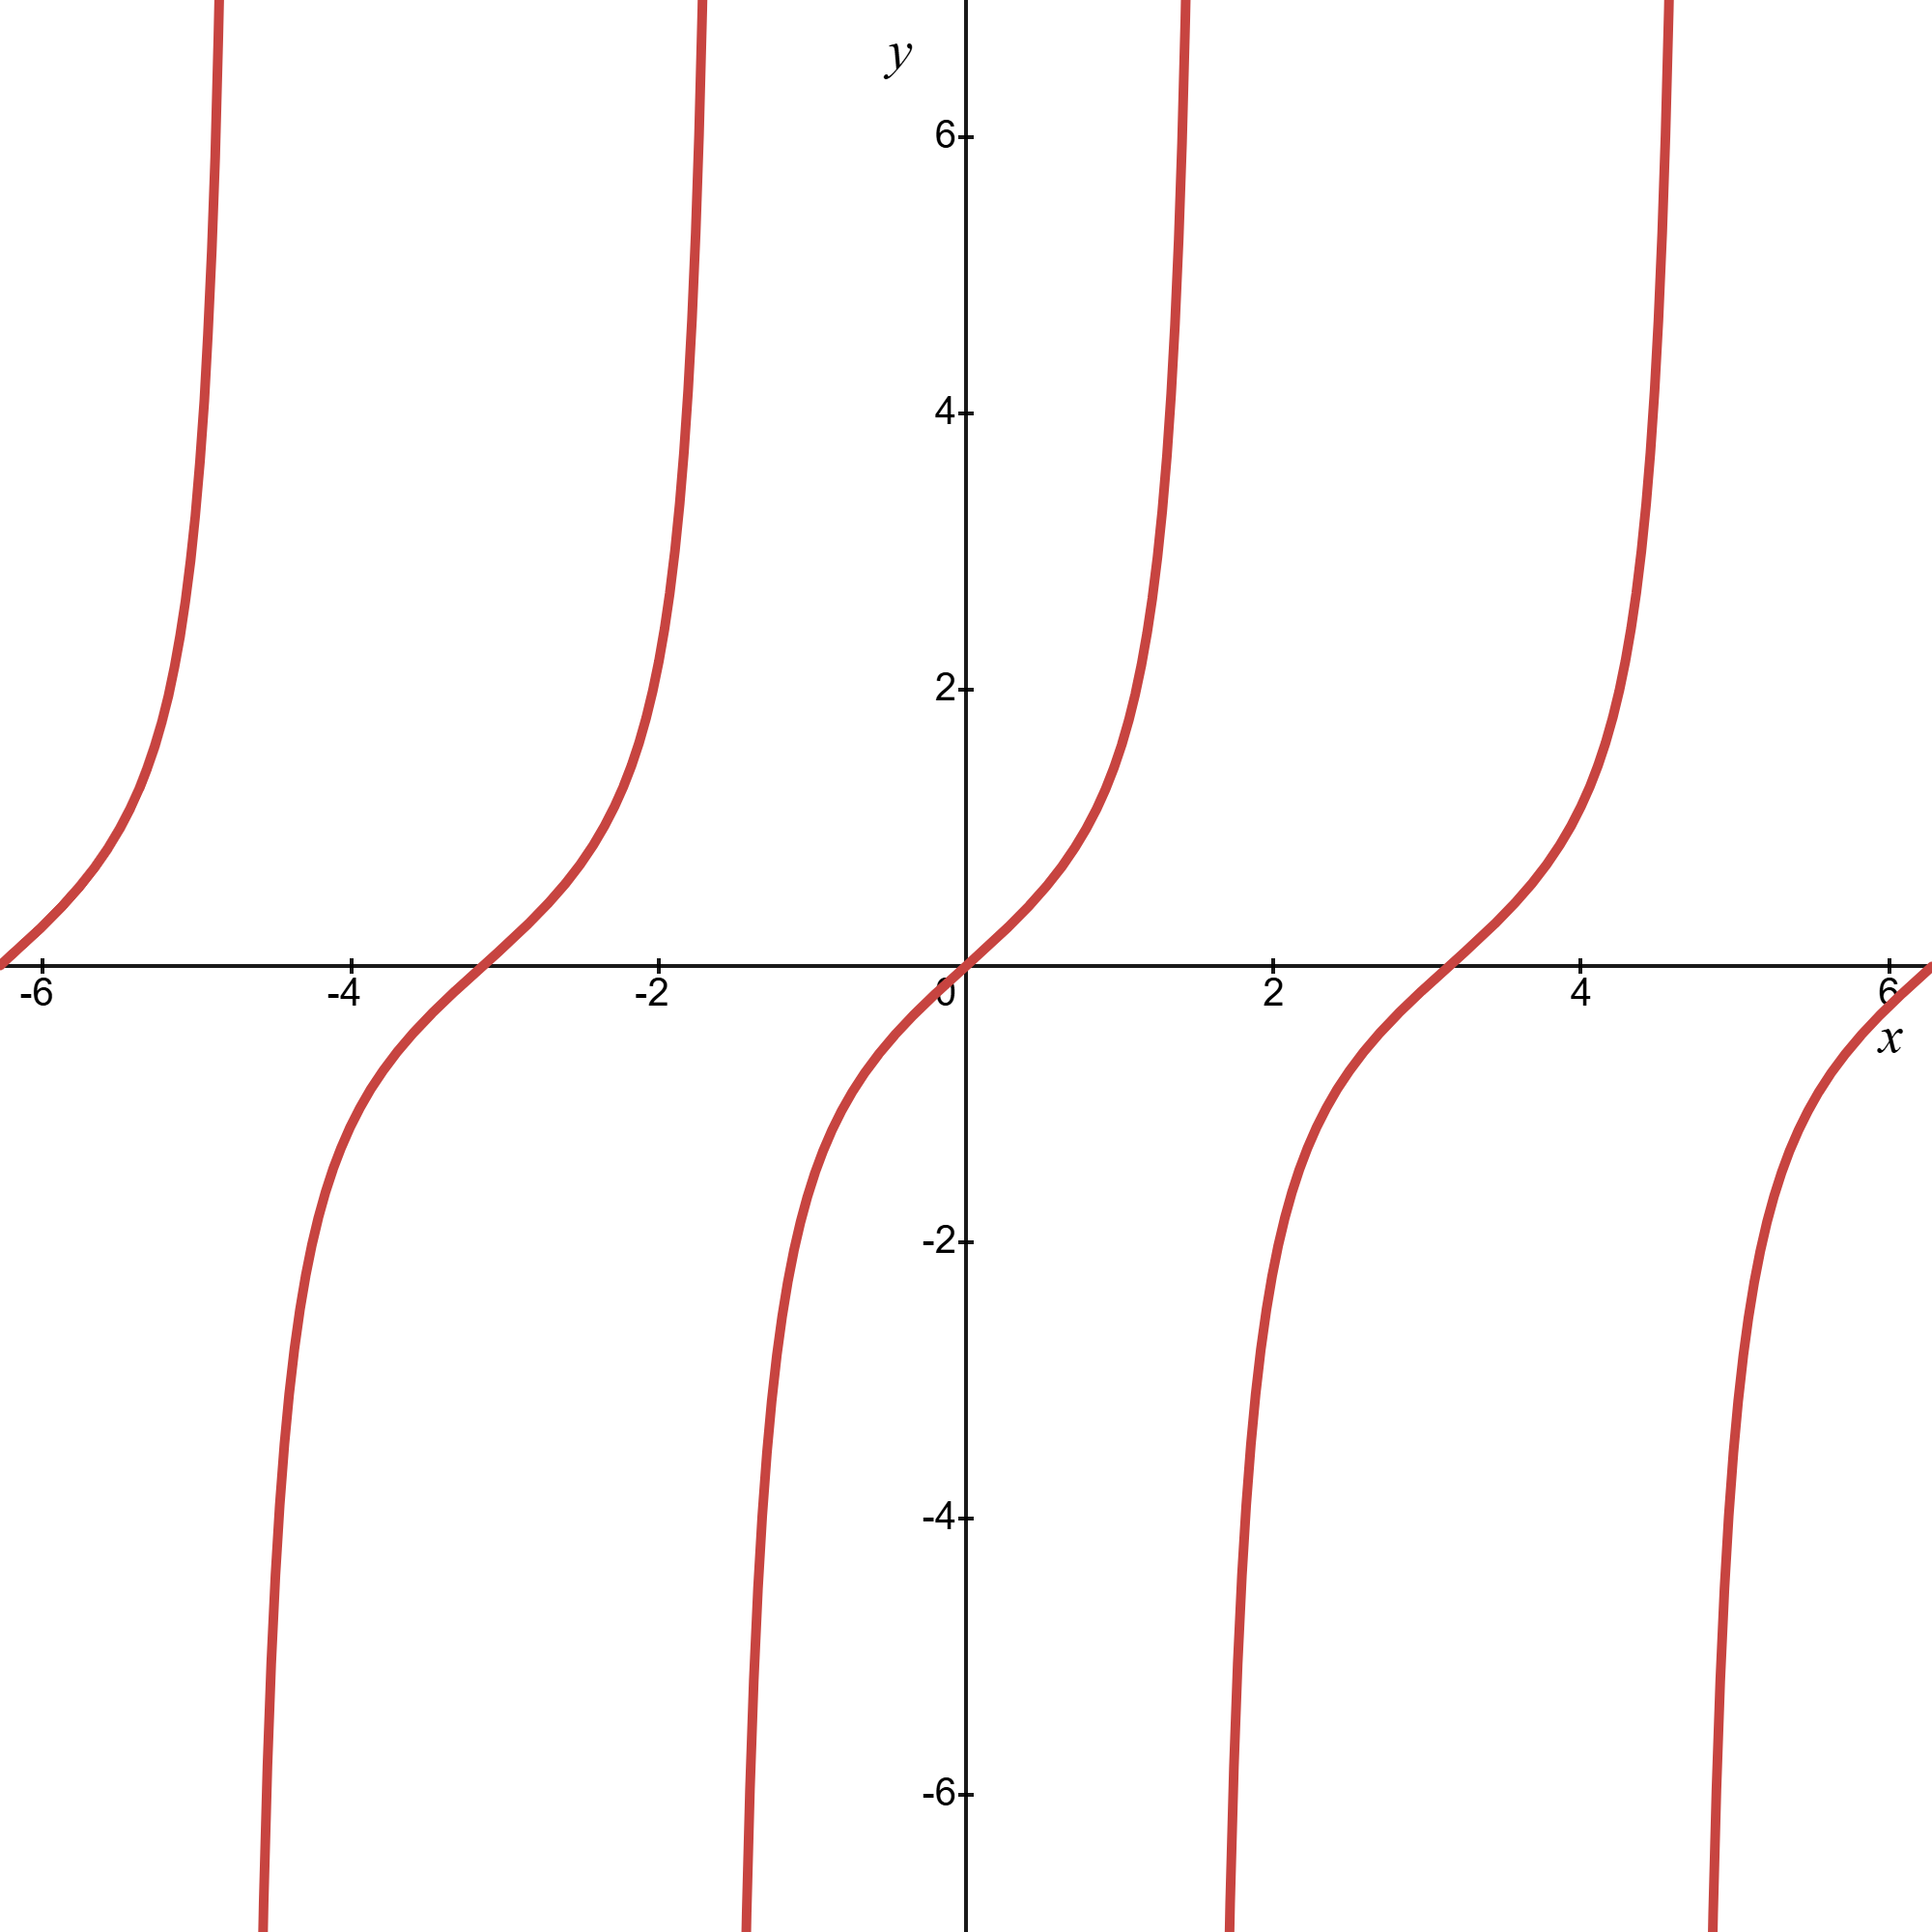
\includegraphics[width=0.45\textwidth, alt ={Graph of a tan(x).}]{figures/tan_graph}
  %}{A plot of the tan function. }
    \caption{A plot of the trig function $\tan(x)$, unlike $\sin$ and $\cos$ above, $\tan$ cannot be drawn without taking your pen off the page.  }
\label{fig: tan function}
\end{figure}

The trig functions are clearly not one-to-one, since they are periodic, in fact even restricted to $x\in[0,2\uppi)$ there are repeated values. However, just like with the square root, it is convenient to introduce inverse functions, where we need to be careful which quadrant our angle is in to get a single value out. These inverse functions are often denoted
\begin{align*}
\sin^{-1}(x)&=\arcsin(x),\\
\cos^{-1}(x)&=\arccos(x),\\
\tan^{-1}(x)&=\arctan(x).
\end{align*}

Your calculator will have a button for each trig function, and a way to select the inverse functions, typically calculators return answers in the following ranges:
\begin{equation*}
0\leq \arccos(x)\leq \uppi,\qquad -\frac{\uppi}{2}\leq \arcsin(x)\leq \frac{\uppi}{2}, \qquad -\frac{\uppi}{2}< \arctan(x)< \frac{\uppi}{2}.
\end{equation*}

The inverse trig functions are useful if we need to solve equations involving trig functions.\\

\begin{ex}
Find the solutions to $4\cos(t)=3$ for $t\in[-8,10]$. \\

The first step is to divide both sides by $4$ to give us
\begin{equation*}
\cos(t)=\frac{4}{3},
\end{equation*}
now we can use
\begin{equation*}
t=\arccos\left(\frac{3}{4}\right)=0.7227.
\end{equation*}

Not that this is just one of an infinite\footnote{``Why infinitely many?'' you ask. This is because $\cos(x)$ is $2\uppi$ periodic so if $t$ is a solution in the range $[0,2\uppi)$ then $t+2\uppi n$ is another solution for $n\in \Z$. } number of solutions to the above equation. in the range from $0$ to $2\uppi$ there are two solutions, $t=0.7227$ and $t=2\uppi-0.7227=5.5605$. We now add $2\uppi n$ to both of our values, testing values of $n$ so that the result stays within the interval :
%\begin{align*}
%&n=-2 \quad t=0.7227-4\uppi = \sout{-11.8437} \quad \text{and} \quad 5.5605-4\uppi=-7.0059\\
%&n=-1 \quad t=0.7227-2\uppi = -5.5605\quad \text{and} \quad 5.5605-2\uppi=-0.7227\\
%&n=0 \quad t=0.7227\quad \text{and} \quad 5.5605\\
%&n=1 \quad t=0.7227+2\uppi = 7.0059 \quad \text{and} \quad 5.5605+2pi=\sout{11.8437}
%\end{align*}

\begin{itemize}
%\setlength{\itemsep}{-5pt}
    \item $n=-2$  then $ t=0.7227-4\uppi =\cancel{-11.8437}$ and $t=5.5605-4\uppi=-7.0059$,
    \item $n=-1$ then $ t=0.7227-2\uppi = -5.5605$ and $t=5.5605-2\uppi=-0.7227$,
    \item $n=0$ then $t=0.7227$ and $t=5.5605$,
    \item $n=1$  then $t=0.7227+2\uppi = 7.0059$ and $ t=5.5605+2\uppi=\cancel{11.8437}$.
\end{itemize}
Thus there are six solutions in the interval $[-8,10]$,
\begin{equation*}
t=-7.0059, -5.5605, -0.7227, 0.7227, 5.5605, 7.0059.
\end{equation*}
Not that the solutions come in positive and negative pairs.
\end{ex}

You will have the opportunity to practice more problems like this either by going through the week one tutorial sheet or by looking at Section 1.5 in \citep{calcI}.\\

The trig functions satisfy some nice relationships that you should try to learn, and which we quote here without any proof. Some of these are fairly easy to prove and are left as an exercise, while others are harder and can be looked up if you are curious.\\

The first one is that 
\begin{equation*}
\tan(x)=\frac{\sin(x)}{\cos(x)}.
\end{equation*}

\paragraph{Squares:} The squares of trig functions have the nice property that
\begin{equation*}
\sin^{2}x+\cos^{2}x =1,
\end{equation*}
which is a consequence of Pythagoras' theorem.

\paragraph{Multiple angles:} There are some very useful identities when we consider trig functions for the sum and difference of an angle:
\begin{align*}
\sin\left(x\pm y\right)&=\sin x \cos y \pm \cos x \sin y,\\
\cos\left(x\pm y\right)&=\cos x \cos y \mp \sin x \sin y.
\end{align*}
For the special case of $x=y$ this leads to 
\begin{align*}
\sin 2x &= 2\sin x \cos x,\\
\cos 2x &=\cos^{2}x-\sin^{2}x = 2\cos^{2}x -1 =1-2\sin^{2}x.
\end{align*}

You should try to become familiar with these identities, at least for this module, as they will be useful wherever trig functions appear.\\

\paragraph{Further trig functions:} There are three more trig functions that you should be aware of. Again, these are not independent trig functions but are one over the familiar trig functions. These are:
\begin{align*}
\sec x &=\frac{1}{\cos x},\\
\csc x &=\frac{1}{\sin x},\\
\cot x &=\frac{1}{\tan x}.
\end{align*}
Plots of these three functions are shown in \cref{fig: sec function}.

\begin{figure}[ht]
    \centering
  %  \pdftooltip{
  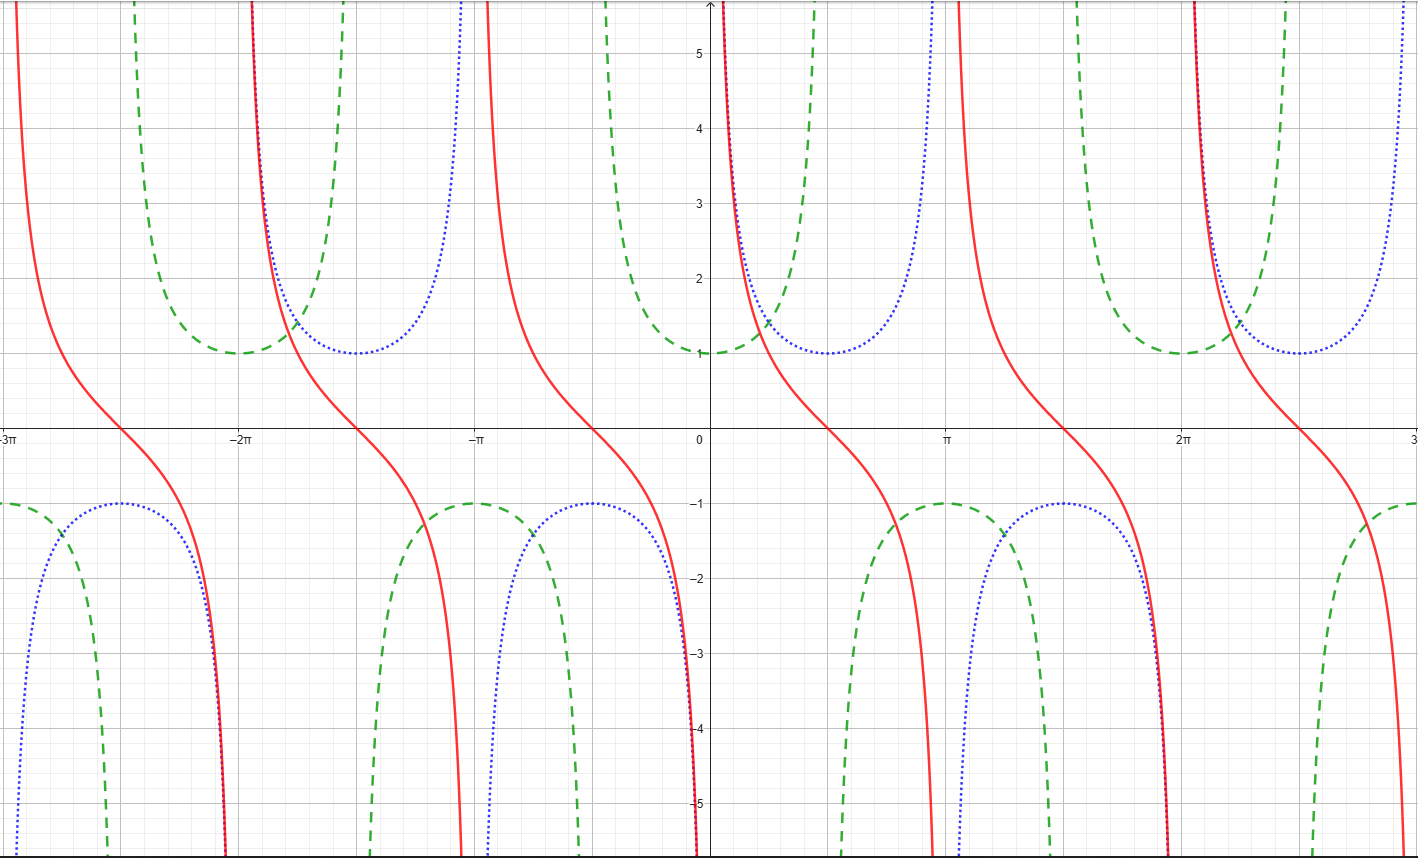
\includegraphics[width=0.8\textwidth, alt ={Graphs of sec(x), csc(x), and cot(x).}]{figures/sec-cot-csc-fig}
  %}{A plot of the other trig function. }
    \caption{A plot of the trig functions produced using GeoGebra: $\sec(x)$ the green dashed line, $\csc(x)$ the blue dotted line, and $\cot(x)$ the solid red line. It is not possible to draw any of these functions without taking the pen off the page, we will see later that this is because these functions have vertical asymptotes where the functions head off to infinity.  }
\label{fig: sec function}
\end{figure}

\section{Logarithms and Exponentials}
\label{sec: log and exp}

Another pair of very useful functions which we need to be familiar with are the logarithm and the exponential function. \\

In your previous maths courses you may have come across the fact that we call powers exponents, e.g. in an expression $f(x)=x^{b}$ then $b$ is called the exponent,, or the index. An exponential function is then a function like
\begin{equation*}
f(x)=b^{x},
\end{equation*}
where a constant\footnote{here $b>0$ and $b\neq 1$.} $b$ is raised to the power of the variable $x$. In this case the number $b$ is called the \textbf{\gls{base}} of the exponential function.\\

The exponential function with base $2$ is shown in \cref{fig: exp and log 1}.  It turns out that by appropriate scaling of $x$ different bases are related\footnote{To get an idea of this consider that $2^{x}=4^{x/2}$ so we can always transform from base $2$ into base $4$. In general we need to use the logarithm function that we will meet shortly.} so we only need one standard basis. \\

When working with binary the basis $b=2$ is chosen, while in scientific notation $b=10$ is chosen.  Nowadays the basis in general use is denoted $e$ or $\exp$ with $\exp(x)$ called the \textbf{exponential function}. \\

\begin{mdiv}
\textbf{Warning}! When talking to mathematicians there is a difference between $e$ and $\exp$, the first one is a number, close to $2.71828\dots$, while $\exp$ is a function. Often we will use $e^{x}$ and $\exp(x)$ interchangeably, but occasionally it is important to know the difference.  The main difference is that $\exp(x)$ is a one-to-one function, in particular  when $x=1/2$ we have that $\exp(1/2)\simeq 1.65$ while when taking $\sqrt{e}=e^{1/2}$ we need to pick either the positive or negative square root.  Most likely you can just forget this distinction and work with $e^{x}$ and $\exp(x)$ as if they were the same thing. However, it is worth seeing the distinction at least once.
\end{mdiv}

\begin{figure}[ht]
    \centering
\ThisAltText{Graph of exponential and logarithm functions with base 2.}
 %   \pdftooltip{
    \begin{tikzpicture}[line width=1pt,line cap=round,line join=round, smooth,variable=\x]
     \draw[->] (-3.8,0) -- (5,0) node[above] {$x$};
  \draw[->] (0,-4) -- (0,5)node[above]{$y$};
 \draw[color=CDnavy, domain=-3.8:2.3]   plot[samples=300] (\x,{2^(\x)}) node[right] {$2^{x}$};
  \draw[color=CDgreen, domain=0.06:4]   plot[samples=300] (\x,{log2(\x )}) node[anchor = north west] {$\log_2(x)$};
  \draw[ dashed, color = gray, domain = -2.5:4.5] plot (\x,\x)node[right]{$y=x$};
    \end{tikzpicture}
%    }{plots of an exponential and logarithm }
    \caption{Plots of the exponential and logarithm functions, $y=2^{x}$ and $y=\log_{2}(x)$.}
        \label{fig: exp and log 1}
\end{figure}

The reason for picking $e$ as the basis is that simplifies some of the algebra associated with exponential functions, it also has the advantage that the tangent to the curve has gradient $1$ at $x=0$. This last part boils down to 
\begin{equation}
e\simeq \left(1+h\right)^{\frac{1}{h}} 
\label{eq: exp approximation}
\end{equation}
for $h$ close to zero. 

\begin{figure}[ht]
    \centering
\ThisAltText{Graph of exponential and logarithm functions with base e.}
%    \pdftooltip{
    \begin{tikzpicture}[line width=1pt,line cap=round,line join=round, smooth,variable=\x, ]
     \draw[->] (-3.6,0) -- (5,0) node[above] {$x$};
  \draw[->] (0,-4) -- (0,5)node[above]{$y$};
 \draw[color=CDnavy, domain=-3.8:1.6]   plot[samples=300] (\x,{exp(\x)}) node[right] {$\exp(x)$};
  \draw[color=CDgreen, domain=0.03:4]   plot[samples=300] (\x,{ln(\x )}) node[anchor = north west] {$\ln(x)$};
  \draw[ dashed, color = gray, domain = -2.5:4.5] plot (\x,\x)node[right]{$y=x$};
    \end{tikzpicture}
%    }{plots of exp and ln }
    \caption{Plots of the exponential and logarithm functions, $y=\exp(x)$ and $y=\ln(x)$.}
        \label{fig: exp and log 2}
\end{figure}

Closely related to $\exp$ is its inverse function, called the \textbf{logarithm} function. You will see it written as either $\log(x)$ or $\ln(x)$, or rarely as $\log_{e}(x)$ where the base is made explicit. \\

As this is an inverse function it is defined as the solution to the equation $e^{y}=x$. For example $e^{y}=4$ is solved by $y=\ln(4)$.\\

The graphs of both $\exp(x)$ and $\ln(x)$ are shown in \cref{fig: exp and log 2}. Note that we are, currently, not defining $\ln$ when $x$ is negative \footnote{If you study more mathematics you will discover that we can make sense of $\ln(x)$ when $x$ is negative. However, it is no longer real and we need to understand complex numbers to make sense of it.}.  You may have guessed that we could take a logarithm in a different basis since it is defined so that
\begin{equation*}
\ln(\exp(x))=x=\exp(\ln(x)).
\end{equation*}

This is why there are several slightly different ways of writing the logarithm. If you learnt about it in school you probably used $\log(x)$ to mean log with base $10$. In this module if we work with a basis other than $e$ we will make this explicit by writing $\log_{b}(x)$ to mean log with base $b$.\\

To be clear $\log_{b}(x)$ is the function defined such that
\begin{equation*}
\log_{b}(b^{x})=x=b^{\log_{b}(x)}.
\end{equation*}

A nice property of exponentials and logarithms is that they map addition to multiplication. What this means is that
\begin{align*}
\exp(a)\exp(b)&=\exp(a+b),\\
\ln(ab)&=\ln(a)+\ln(b),\\
\ln\left(\frac{a}{b}\right)&=\ln(a)-\ln(b).
\end{align*}

Some of the other properties of these functions are that:
\begin{align*}
\exp(-x)&=\frac{1}{\exp(x)},\\
\exp(x)&>0,\\
\exp(x)&\to \infty \quad \text{as } x\to \infty,\\
\exp(x)&\to 0 \quad \text{as } x\to -\infty,\\
\ln(x) &\to \infty \quad \text{as } x\to \infty,\\
\ln(x)&\to -\infty \quad \text{as } x\to 0^{+}.
\end{align*}
We will return to discussing limits shortly, but here the statement $\exp(x)\to \infty$ as $x\to \infty$ means that the function $\exp(x)$ becomes infinitely large as $x$ becomes infinitely large. The terminology for this is that $\exp(x)$ \textbf{diverges} as $x$ tends to infinity.\\

The final, useful, identity about logarithms is how to change the basis. The change of basis formula is
\begin{equation}
\log_{b}(x)=\frac{\log_{a}(x)}{\log_{a}(b)}.
\label{eq:log change of base}
\end{equation}

As with trig functions in \cref{sec: trig func}, $\ln$ and $\exp$ are useful when solving equations. There are lots of examples in \citep{calcI} but we will go through a couple of examples here, there will be more on the tutorial sheets.

\begin{ex}
Consider the equation
\begin{equation*}
x e^{-x} -x =0.
\end{equation*}
The first step in solving this is to factor out the $x$ common to both terms. Note that we \textbf{cannot} divide by $x$ as at this stage we do not know if it will be zero. This gives us
\begin{align*}
x e^{-x} -x &=0\\
x\left(e^{-x}-1\right)&=0,
\end{align*}
so we get two possibilities\footnote{Sometimes we will get more than two possibilities, remember with trig functions their periodicity meant that we had infinitely many solutions.}: either $x=0$ or $e^{-x}-1=0$. If we had divided by $x$ we would have missed that $x=0$ is a solution, and would not have completely solved the problem. Consider the second case,
\begin{align*}
e^{-x}&=1\\
-x&=\ln(1)=0
\end{align*}
so this other case also reduces to $x=0$ and we only have one solution in this case.
\end{ex}

\begin{ex}
\label{ex: log equation}
Consider the equation
\begin{equation*}
\frac{1}{2}\ln\left(x^{2}\right)-\ln\left(x-1\right)=4.
\end{equation*}
If we make use of the log rules we have that $\ln(x^{2})/2=\ln(\sqrt{x^{2}})=\ln x$, where we take the positive square root as currently we do not know how to make sense of logarithms with negative arguments. The equation thus becomes
\begin{align*}
4&=\frac{1}{2}\ln\left(x^{2}\right)-\ln\left(x-1\right)\\
&=\ln\left(x\right)-\ln\left(x-1\right)\\
&=\ln\left(\frac{x}{x-1}\right).
\end{align*}
Now we can exponentiate both sides and rearrange to solve for $x$:
\begin{align*}
\frac{x}{x-1}&=e^{4}\\
x&=e^{4}\left(x-1\right)\\
x&=-e^{4}+xe^{4}\\
x\left(1-e^{4}\right)&=-e^{4}\\
x&=-\frac{e^{4}}{1-e^{4}}=1.01866.
\end{align*}

When we get an answer like this we need to check that it does not give a negative argument in any of the original logarithms, here we are fine since both $x^{2}$ and $x-1$ are positive.

\end{ex}

It may seem like example~\ref{ex: log equation} took quite a bit of working out, but with practice you will get faster at solving problems like this. In the lectures you will frequently hear me paraphrasing George P\'{o}lya and saying that Mathematics is not a spectator sport. This means that while reading these notes and attending the lectures can help you in your learning there is no substitute for actually rolling your sleeves up and solving problems. Remember that most modules \textit{expect} you to be putting in around three hours of self study for every hour of contact time.

\section{Hyperbolic functions}
\label{sec: hyperbolic functions}
The next class of functions that it is useful to know about are the \textbf{hyperbolic} trig functions. As shown in \cref{fig: hyperbolic functions}, the hyperbolic trig functions are the analogue of the standard trig functions of \cref{sec: trig func} but adapted to the geometry of the hyperbola, $x^{2}-y^{2}=1$ rather than the circle $x^{2}+y^{2}=1$. For the standard trig functions, their argument was an angle related to how far round the unit circle we had gone. In the hyperbolic case the \textit{angle} is now twice the shaded area shown in \cref{sec: trig func}. \\

\begin{figure}[ht]
    \centering
  %  \pdftooltip{
  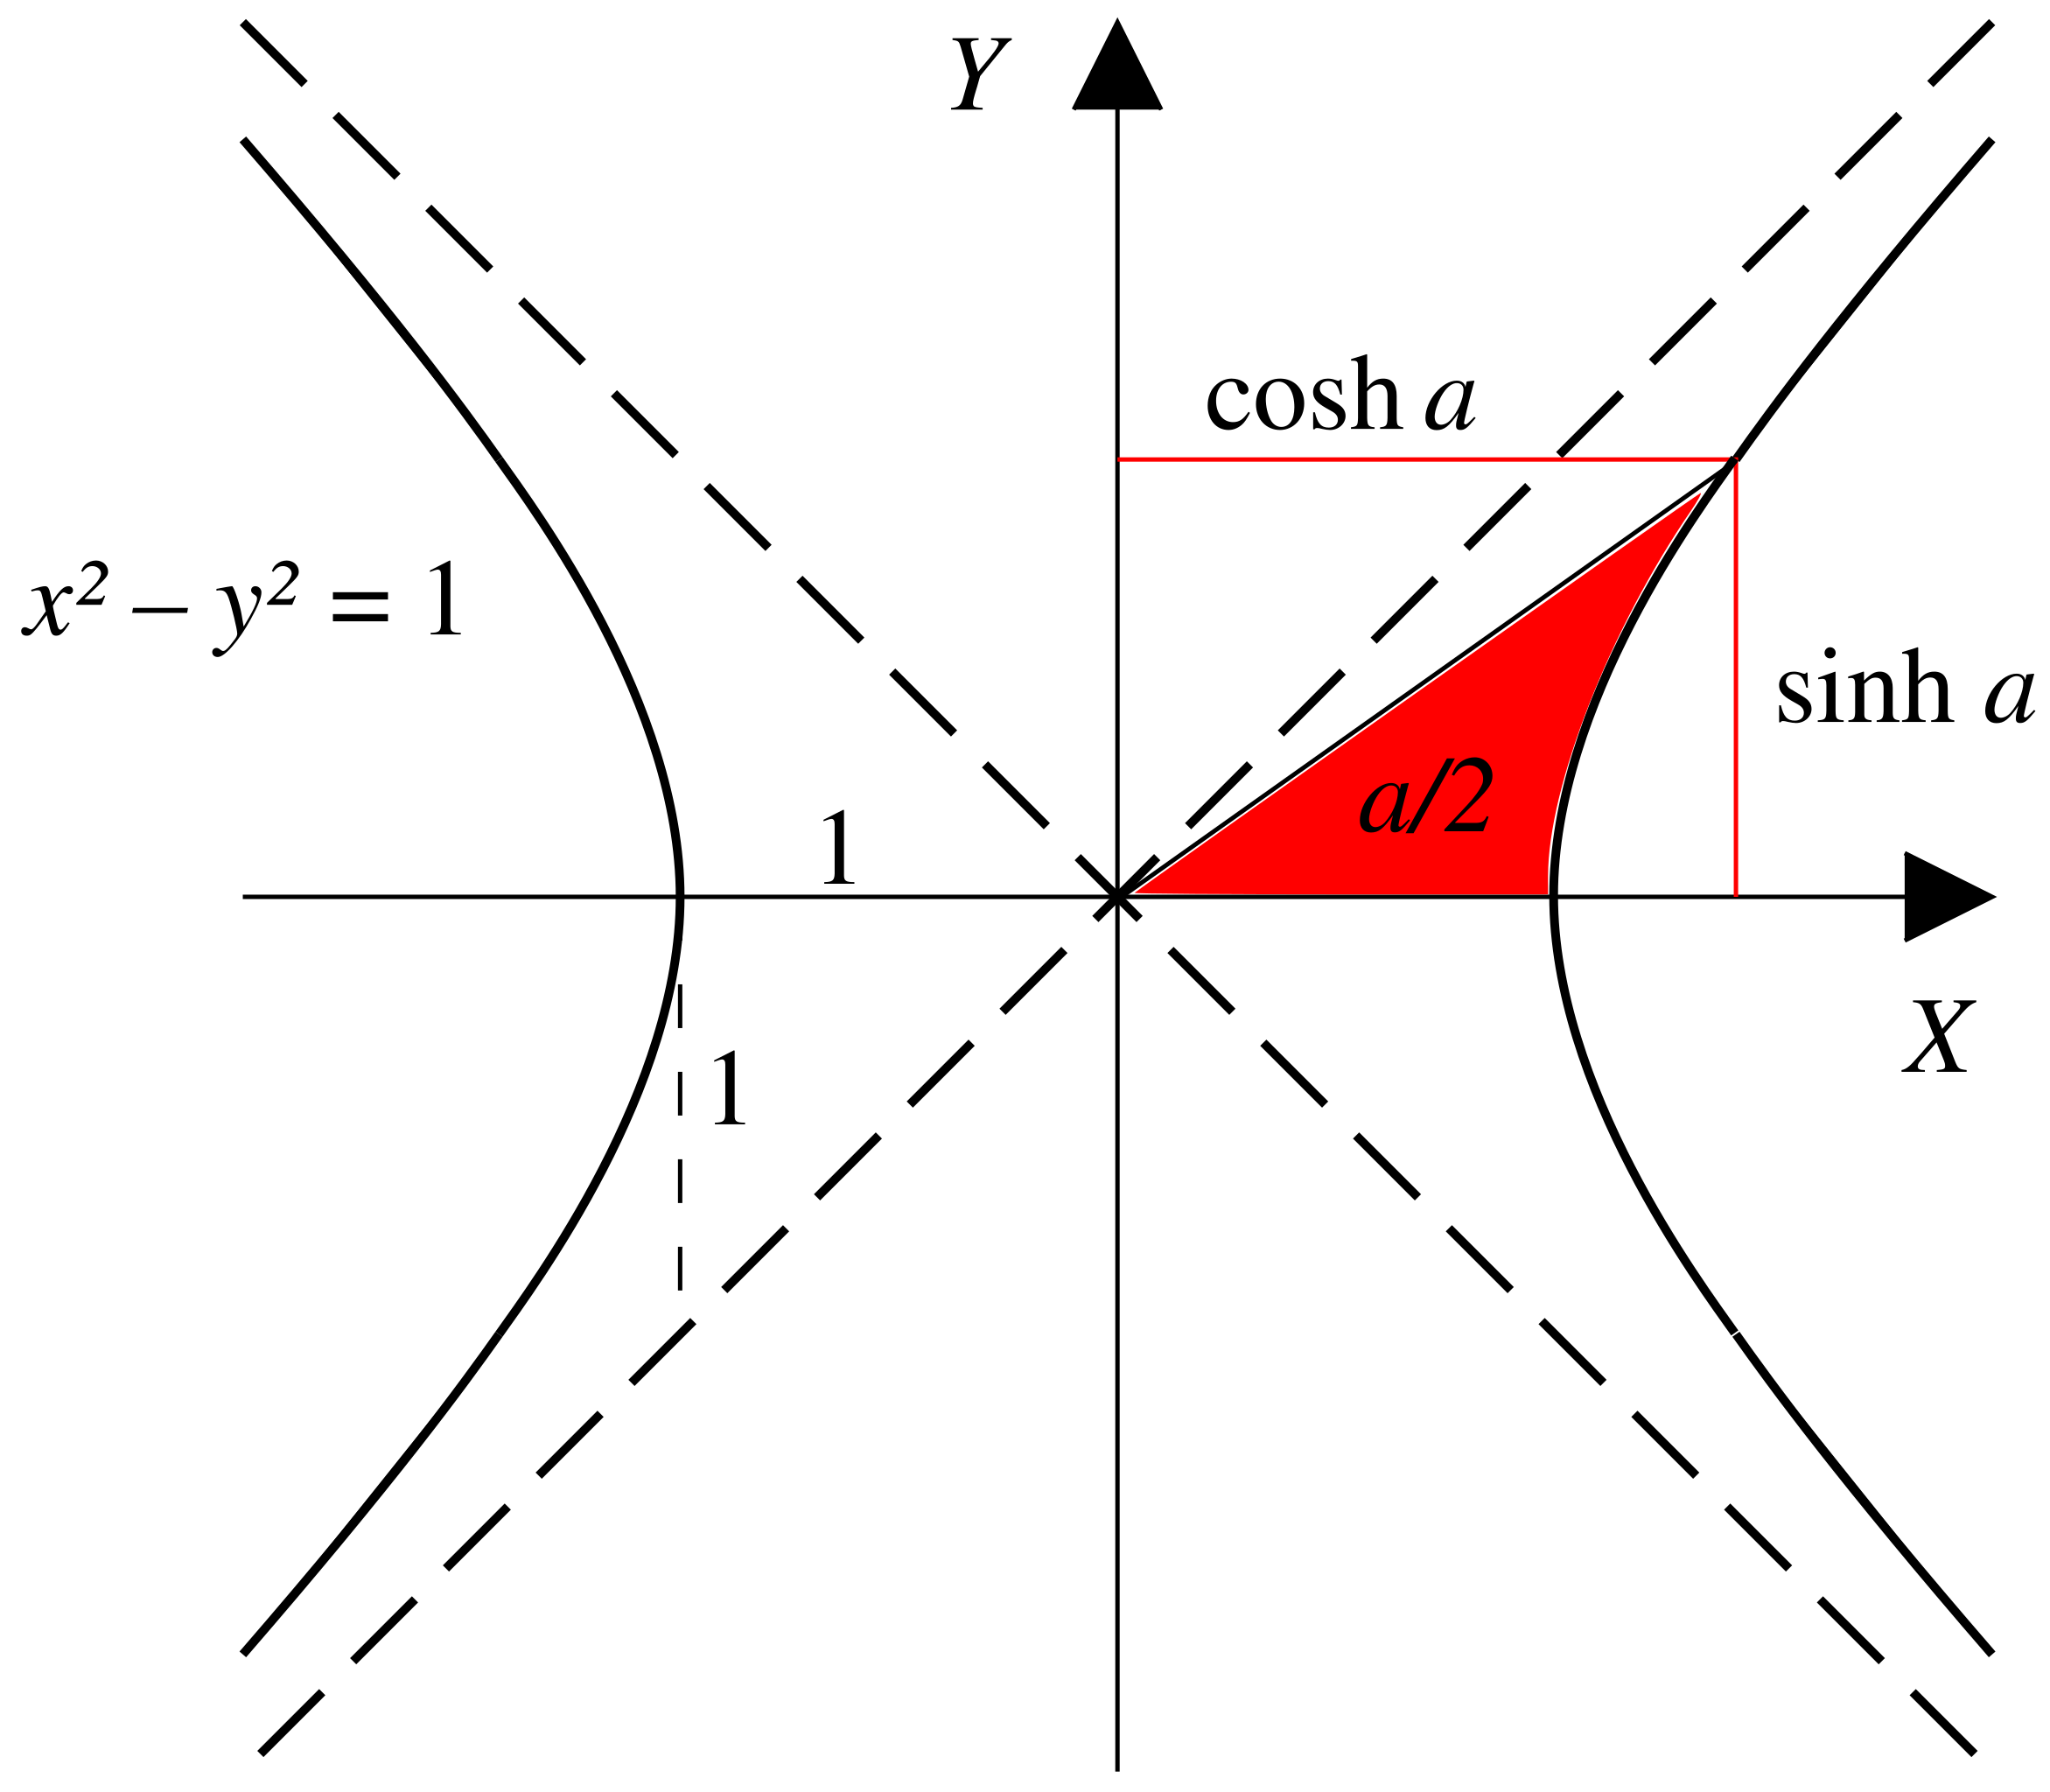
\includegraphics[width=0.4\textwidth, alt ={Hyperbolic trig functions are related to the geometry of hyperbolas rather than circles.}]{figures/Hyperbolic_functions}
  %}{A plot of the tan function. }
    \caption{Hyperbolic trig functions are defined in terms of  the area enclosed by a radial ray and the hyperbola $x^{2}-y^{2}=1$.  The convention is to assume that $a$ is negative for points below the $x$-axis. The image is from \href{https://commons.wikimedia.org/wiki/File:Hyperbolic_functions-2.svg}{Wikimedia commons}. }
\label{fig: hyperbolic functions}
\end{figure}


There is a hyperbolic equivalent of all of the standard trig functions, and the notation is very similar just with an added $h$ at the end:
\begin{itemize}
%\setlength{\itemsep}{-5pt}
    \item \textbf{hyperbolic sine}  $\sinh$,
    \item \textbf{hyperbolic cosine} $\cosh$,
   \item \textbf{hyperbolic tangent} $\tanh$,
   \item \textbf{inverse hyperbolic sine} $\arcsinh$,
   \item \textbf{inverse hyperbolic cosine} $\arccosh$,
   \item \textbf{inverse hyperbolic tangent} $\arctan$.
\end{itemize}
There are also hyperbolic versions of the other trig functions but we will not be as concerned with them here.\\

As in the regular trig case the hyperbolic tangent is defined in terms of the other two functions as
\begin{equation}
\tanh(x)=\frac{\sinh(x)}{\cosh(x)}.
\label{eq: hyperbolic tangent}
\end{equation}

The hyperbolic trig functions are actually defined in terms of the odd and even parts of the exponential function\footnote{If you have come across complex numbers then you may know that this is only true for real $x$, if the argument is imaginary then relationships like this hold between the exponential function and the standard trig functions. We may see this in the advanced topics section of the module if there is enough time.} as follows:
\begin{align}
\sinh(x)&=\frac{e^{x}-e^{-x}}{2}, \label{eq: sinh exp}\\
\cosh(x)&=\frac{e^{x}+e^{-x}}{2}. \label{eq: cosh exp}
\end{align}
They have the following useful properties:
\begin{align*}
\sinh(-x)&=-\sinh(x),\\
\cosh(-x)&=\cosh(x),\\
\cosh^{2}(x)-\sinh^{2}(x)&=1,\\
1-\tanh^{2}(x)&=\sech^{2}(x).
\end{align*}
These are very similar to the identities satisfied by the ordinary trig functions. However, the sign in front of $\sinh(x)$ and $\tanh(x)$ is negative while that in front of $\sin(x)$ and $\tan(x)$ in the equivalent formulae was positive. The rule of thumb when converting from identities for trig functions to identities for hyperbolic trig functions is to send $\cos^{2}(x)\to \cosh^{2}(x)$ and $\sin^{2}(x)\to -\sinh^{2}(x)$.  There are also analogues of the addition of angle identity formulas that you can try to derive if you are interested.\\


\begin{ex}
Consider the hyperbolic equation $\cosh(x)-5\sinh(x)-5=0$ from chapter 3.7 in \citep{riley_mathematical_2006}. The easiest way to solve this is to use the definitions of the hyperbolic functions in terms of the exponential function. This transforms the equation into
\begin{equation*}
\frac{1}{2}\left(e^{x}+e^{-x}\right)-\frac{5}{2}\left(e^{x}-e^{-x}\right)-5=0,
\end{equation*}
which we rearrange to give
\begin{equation*}
0=e^{x}\left(\frac{1}{2}-\frac{5}{2}\right)+e^{-x}\left(\frac{1}{2}+\frac{5}{2}\right)-5=-2e^{x}+3e^{-x}-5.
\end{equation*}
Then multiply through by $-e^{x}$, which is allowed since this is never zero, to get
\begin{equation*}
2e^{2x}+5e^{x}-3=0.
\end{equation*}
Now we could either let $y=e^{x}$ and use the quadratic formula to solve for $y$ or we can factorise this to get
\begin{equation*}
\left(2e^{x}-1\right)\left(e^{x}+3\right)=0,
\end{equation*}
so there are two solutions: $e^{x}=1/2$ or $x=-\ln(2)$, and $e^{x}=-3$ or $x=\ln(-3)$. Remember we have not discussed how to make sense of the logarithm of a negative number so for us there is only one real solution, $x=-\ln(2)$.
\end{ex}

Since the hyperbolic trig functions are related to the exponential function you can probably guess that their inverses are related to the logarithm. It is worth thinking about how to show this relationship. I will show you how to do this for $\sinh(x)$ and $\tanh(x)$ but leave deriving the identify for $\cosh(x)$ as an exercise for the interested reader.

\begin{ex}
Consider $y=\arcsinh(x)$, we can invert this to give $x=\sinh(y)$. Next if we make use of \cref{eq: sinh exp,eq: cosh exp} we have that
\begin{align*}
e^{y}	&=\cosh(y)+\sinh(y)\\
	&=\sqrt{1+\sinh^{2}(y)}+\sinh(y)\\
	&=\sqrt{1+x^{2}}+x.
\end{align*}
Taking $\ln$ of both sides then gives that
\begin{equation}
\arcsinh(x)=y=\ln\left(\sqrt{1+x^{2}}+x\right).
\label{eq: arcsinh log}
\end{equation}
\end{ex} 

If you do a similar calculation for $y=\arccosh(x)$ you will find that
\begin{equation}
\arccosh(x)=\ln\left(x\pm \sqrt{x^{2}-1}\right).
\label{eq: arccosh log}
\end{equation} 

You should think about why there is a $\pm$ in this formula but there was not one in \cref{eq: arcsinh log}.

\begin{ex}
Consider $y=\arctanh(x)$, which inverts to $x=\tanh(y)$. Using the definition of $\tanh(y)$ as being $\sinh(y)/\cosh(y)$ and \cref{eq: sinh exp,eq: cosh exp}  we have that
\begin{equation*}
x=\frac{e^{y}-e^{-y}}{e^{y}+e^{-y}}
\end{equation*}
which is equivalent to 
\begin{equation*}
\left(x+1\right)e^{-y}=\left(1-x\right)e^{y}.
\end{equation*}
which can be further rearranged to give
\begin{align*}
e^{2y}&=\frac{1+x}{1-x},\\
\Rightarrow e^{y}&=\sqrt{\frac{1+x}{1-x}},\\
y&=\ln\left(\sqrt{\frac{1+x}{1-x}}\right).
\end{align*}
This gives that 
\begin{equation}
\arctanh(x)=\frac{1}{2}\ln\left(\frac{1+x}{1-x}\right).
\label{eq: arctanh log}
\end{equation} 

\end{ex}

You may be asking why we have spend the time deriving these identities for the hyperbolic functions, and why we discussed their relationship with the exponential function. This is because when we start to differentiate or integrate hyperbolic functions it is often more straightforward to use the expressions involving exponentials and logarithms. 


\section{Limits and asymptotics}
We have now spent quite a bit of time discussing different examples of functions and their properties, as well as how to plot them. If we consider the plot of the tangent function in \cref{fig: tan function} you may have asked at the time, what happens when the red line goes off the top of the page and reappear at the bottom? If we followed both lines we would see that they are getting closer and closer to the point $x=\uppi/2$. This idea of zooming in on a particular value $x=a$ and asking what happens to a function there is known as \textbf{taking a limit} as $x$ approaches $a$ and is denoted $\lim_{x\to a}f(x)$.\\

If the function is \textit{well behaved} at the point $a$, then the limit is just the value of the function evaluated at $a$, $f(a)$. For example
\begin{equation*}
\lim_{x\to 0}\cos(x)=1=\cos(0).
\end{equation*}
The value of the limit does not have to be finite, it can head off to infinity. A good example of this is the exponential function which just keeps getting larger as $x$ increases. We denote this by
\begin{equation*}
\lim_{x\to \infty}\exp(x)\to \infty.
\end{equation*}
Notice that since the value of the limit is infinite we do not write an equals sign but instead use $\to$ to denote that the limit \textbf{diverges}\footnote{This is just the term that mathematicians use for a function that heads off to infinity.}. There are lots of other examples of functions that diverge, and not always for large $x$. A nice example to have in mind is $y=1/x^{2}$ which diverges as $x\to 0$.\\

In the case of $\tan(x)$ we can observe that $\lim_{x\to \uppi/2}\tan(x)$ will take on different values depending on if $x$ is approaching $\uppi/2$ from above or below. This means that the limit \textbf{does not exist}. In \cref{sec: continuity} we will discuss the consequences of this for the function in more detail. If we are taking the limit from above we often say $x\to a^{+}$, while the limit from below is denoted $x\to a^{-}$. In this case
\begin{align*}
\lim_{x\to \frac{\uppi}{2}^{+}}\tan(x)&\to \infty,\\
\lim_{x\to \frac{\uppi}{2}^{-}}\tan(x)&\to -\infty,
\end{align*}
so $\tan(x)$ diverges in different directions depending on how we approach $\uppi/2$.

\begin{mdiv}
Putting our mathematician's hats on for a brief moment, we would say that limit of a function $f(x)$ as $x$ approaches $a$ is $L$ and write it as
\begin{equation*}
\lim_{x\to a}f(x)=L,
\end{equation*}
as long as we can make $f(x)$ as close to $L$ as we want for all $x$ sufficiently close to $a$ on both sides, without taking $x=a$.\\

If this was a maths module we would be even more precise and give what is called an $\upepsilon,\updelta$ definition. Fortunately for all of us this is not a maths module and we can focus on a more practical/ working  definition rather than getting bogged down in the abstract details. If you are interested to know how to do this in detail, the section ``The Definition of a Limit'' in \citep{calcI} is a good place to look.  \\

\textbf{Remember} that $x\to a$ does not mean that $x$ becomes equal to $a$, it just means that $x$ is getting close to $a$. It is also possible that $f(x)$ may never equal $L$, but also just get close to it. This is especially true when we take the limit  near a point that the function is not defined at, e.g. $x\to \uppi/2$ for $\tan(x)$.
\end{mdiv}

Curve sketching is a useful way to understand the main features of a function and can help us to know if the limit exists and if we have the same limit when approaching from different directions. 

\begin{ex}
Consider the function 
\begin{equation}
f(x)=\frac{1}{x-2},
\label{eq: reciprocal of x-2}
\end{equation}
defined for $x\neq 2$.\\

Notices that for $x\to\pm \infty$ $f(x)\to 0$, in \cref{fig: asymptotes function} we see that the plot approaches the horizontal axis \textbf{asymptotically}\footnote{The definition of asymptotically is ``approaching a given value or condition, as a variable or an expression containing a variable approaches a limit, usually infinity'' \citep{collins:asymptotically}}. We can also observe that for $a\neq 2$ $f(x)\to f(a)$ for $x\to a$.  The only point where we need to be careful is when $x$ tends to $2$ looking at \cref{fig: asymptotes function} we see that if we approach $2$ from above that $f(x)\to \infty$ while if we approach $2$ from below $f(x)\to -\infty$. \\

Note that the fact that $f(x)$ is not defined at $x=2$ has no bearing on the limiting behaviour.

\end{ex}

\begin{figure}[ht]
    \centering

  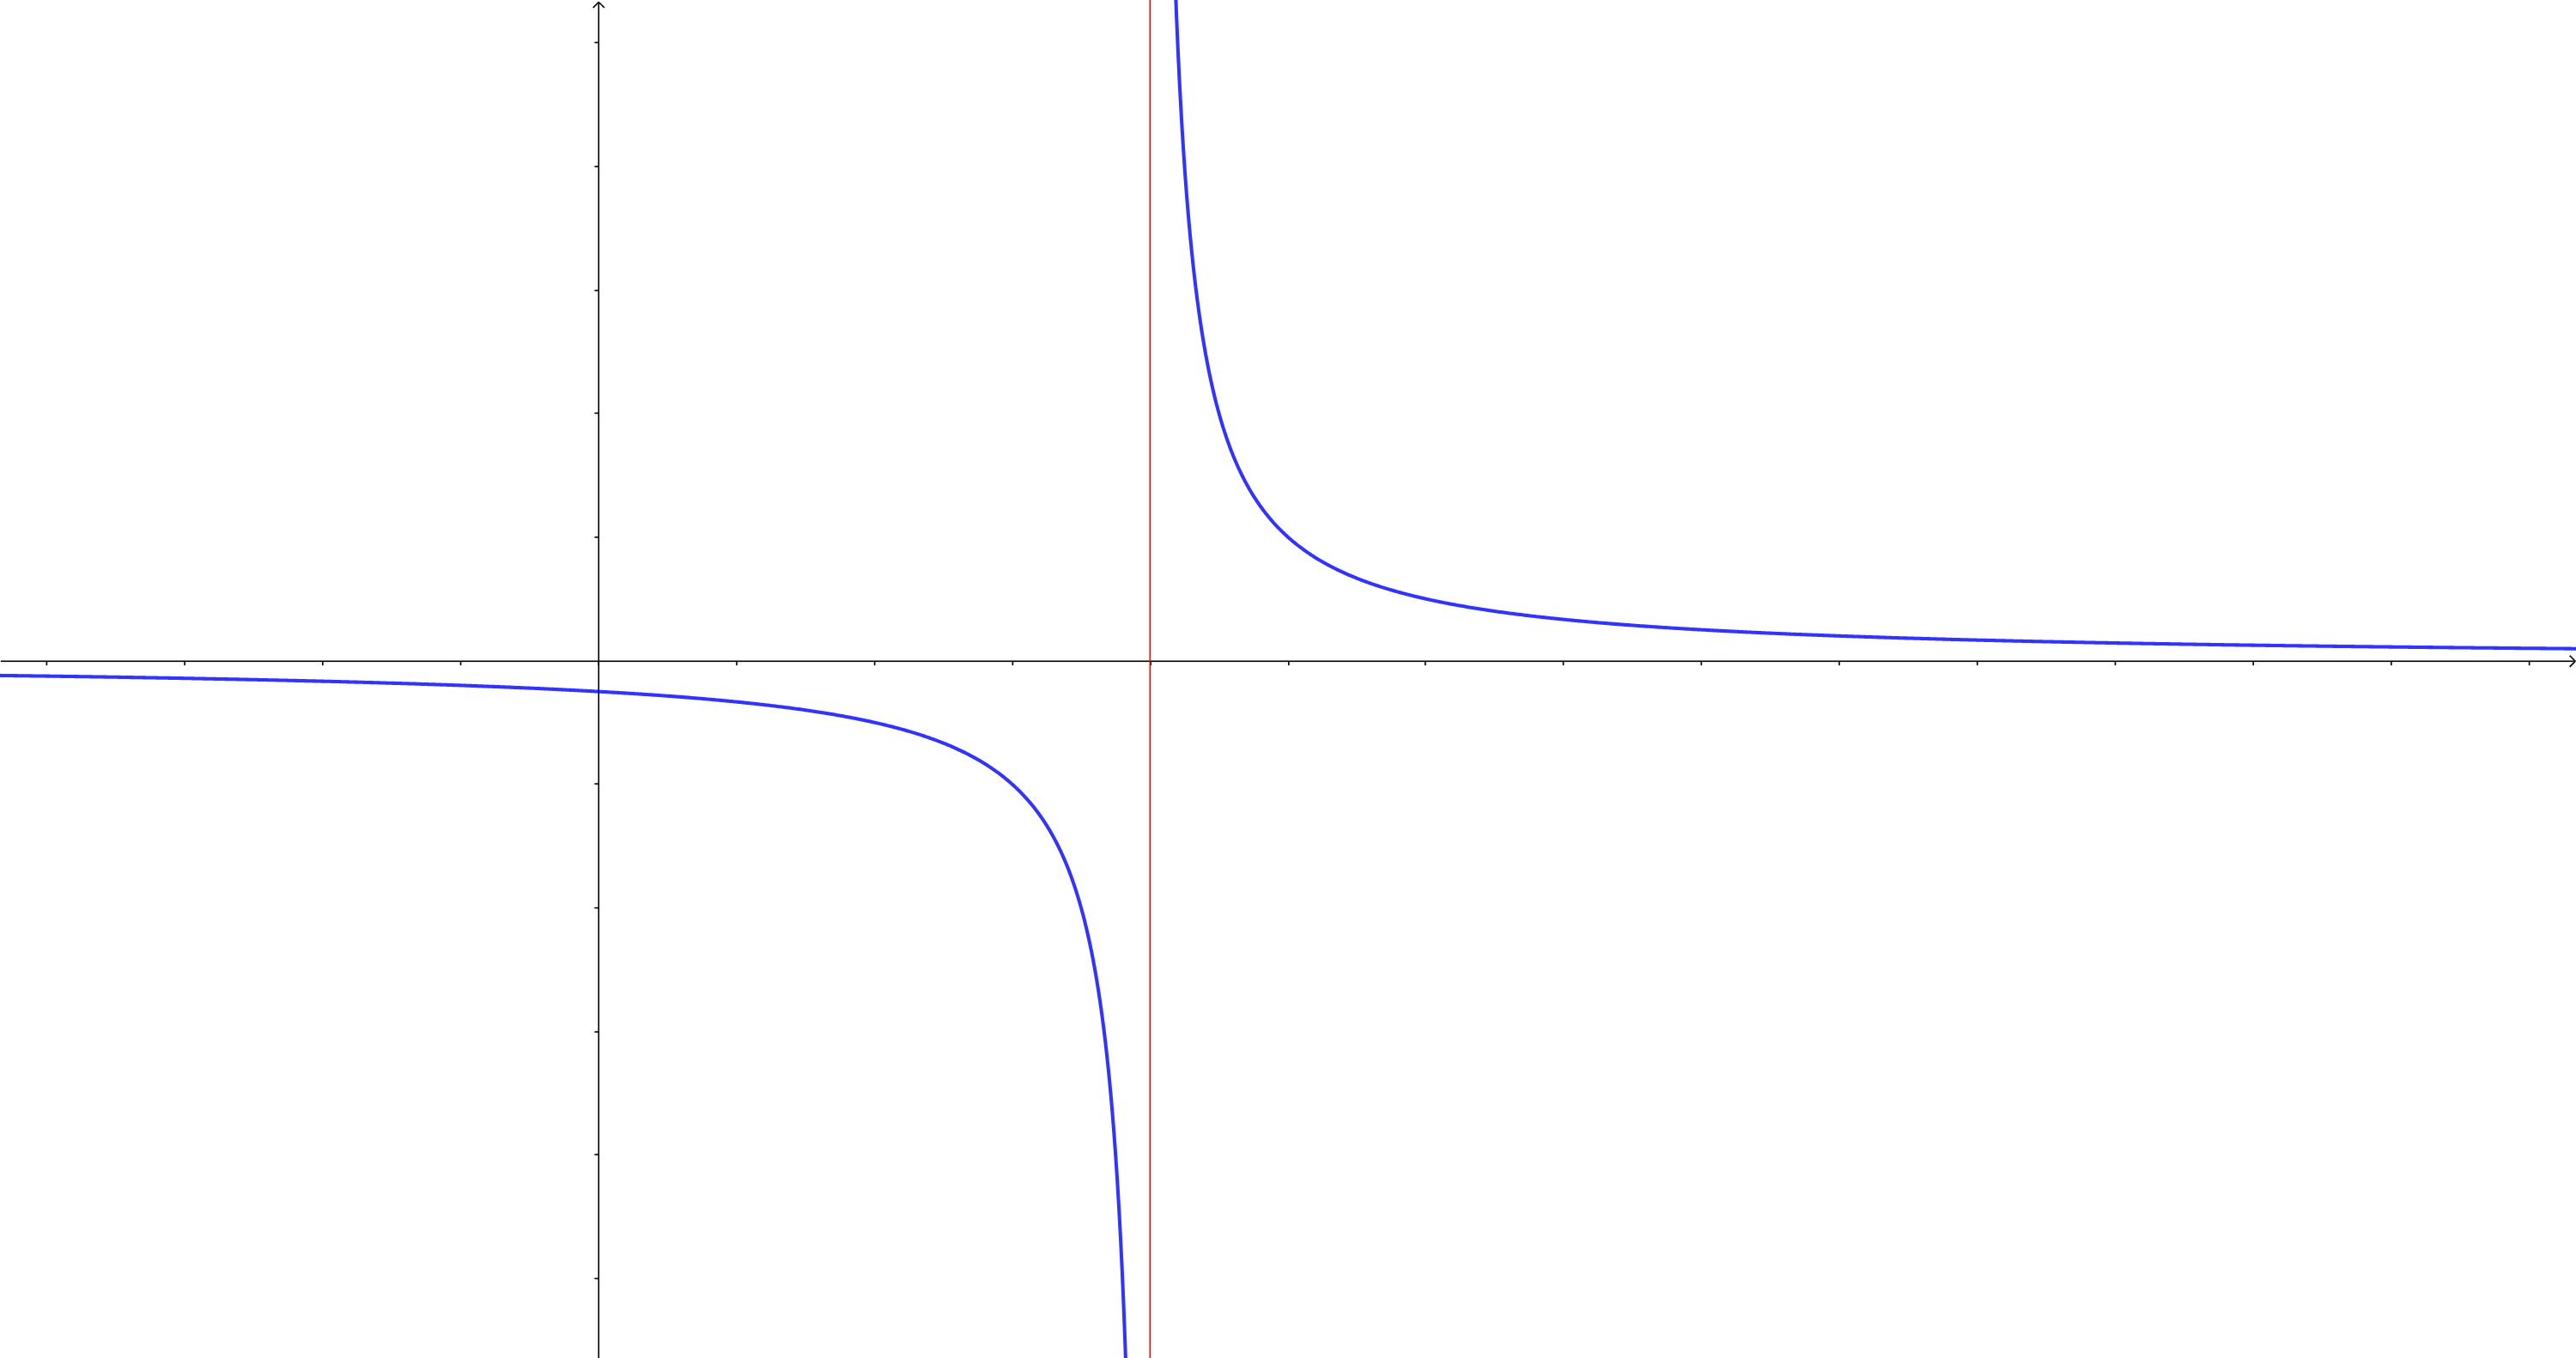
\includegraphics[width=0.6\textwidth, alt={A plot of the reciprocal of (x-2) which tends to zero as x goes to either plus or minus infinity and diverges as x tends to 2.}]{figures/asymptotes}
    \caption{A plot of the function from \cref{eq: reciprocal of x-2} produced using GeoGebra. The blue line is the function and the red line shows where the function diverges and has a vertical asymptote.}
\label{fig: asymptotes function}
\end{figure}

The general rule when curve sketching is to set $y=f(x)$ for the function of interest $f(x)$, and then to investigate the following:
\begin{itemize}
%\setlength{\itemsep}{-5pt}
    \item The \textbf{intercepts} of $f(x)$, these are the points where the function meets or crosses the coordinate axes, e.g. $f(x=0)$ and $f(x)=0$, as these position the graph relative to the coordinate axes.
    \item What happens to $y$ as $x\to\pm\infty$?
   \item Which values of $x$ make $y\to \pm\infty$?
   \item Does the function have any \textbf{symmetry}? For example does $f(-x)=f(x)$ ($f$ is even), or $f(-x)=-f(x)$ ($f$ is odd).
   \item Is the function periodic? 
\end{itemize}
Note that a function can have several of these interesting features. e.g. the trig functions are all periodic, while $\sin(x)$ and $\tan(x)$ are odd functions and $\cos(x)$ is an even function.

\begin{mdiv}
An asymptote to a curve is a straight line that becomes close to the curve as either $x$ or $y$ tend to $\pm\infty$. In our above example the curve of \cref{eq: reciprocal of x-2} has two asymptotes, the horizontal $x$-axis for $x\to \pm\infty$ and the vertical line $x=2$ for $x\to 2$.\\

When sketching a curve it is often useful to start by drawing the asymptotes in as they help you to know how the function will behave in certain regions of the plot. In some books you may see $f(x)\asymp mx +c$ as $x\to \infty$ to signify that the straight line $y=mx+c$ is an asymptote to the graph of $f(x)$ as $x$ tends to infinity.
\end{mdiv}

\begin{exercise}
Apply the above rules to produce a sketch of the function
\begin{equation*}
f(x)=\frac{x+2}{x-1}.
\end{equation*}
\end{exercise}

\begin{ex}
Consider the rational function 
\begin{equation*}
f(x)=\frac{x^{2}+4x-12}{x^{2}-2x}
\end{equation*}
and compute its limit as $x\to 2$.

Looking at the function you may think that it will diverge as $x\to 2$ since the denominator vanishes there. However the first step is always to look at if there are any common factors between the numerator and denominator. Factorising both we have
\begin{align*}
f(x)&=\frac{x^{2}+4x-12}{x^{2}-2x}\\
&=\frac{(x+6)(x-2)}{x(x-2)}\\
&=\frac{x+6}{x}.
\end{align*}
So the denominator does not vanish at $x=2$. We can now evaluate the limit to be
\begin{equation*}
\lim_{x\to 2}f(x)=\lim_{x\to 2}\frac{x+6}{x}=\frac{8}{2}=4.
\end{equation*}

The limit is the same regardless of which direction we approach $2$ from.
\end{ex}

\begin{exercise}
Estimate the limit from the above example by constructing a table of values of $x$ and $f(x)$ for $x$ approaching 2 from both above and below.
\end{exercise}

As a warning, this approach of tabulating the values does not work if the function is oscillating. For example, if you try to evaluate the limit as $x\to 0$ of $\cos\left(\uppi/x\right)$ it can look like it is tending to a constant if we are not careful with the values that we pick. However, if we plot the function we see that it is highly oscillatory around zero.

\begin{ex}
Consider the rational function
\begin{equation*}
f(x)=\frac{x^{3}+x^{2}-5x-2}{2x^{3}-7x^{2}+4x+4}.
\end{equation*}
It has three interesting limits, $x\to 0,\infty,2$. We can evaluate the first two of these here, but need to leave the third, $x\to 2$ until we have learnt about L'H\^{o}pital's rule in \cref{sec:advanced topics}. We will do $x\to 0$ first. As usual we check that the numerator and denominator both make sense as $x\to 0$ and then can evaluate the limit
\begin{align*}
\lim_{x\to 0}f(x)&=\lim_{x\to 0}\frac{x^{3}+x^{2}-5x-2}{2x^{3}-7x^{2}+4x+4}\\
&=\frac{-2}{4}\\
&=-\frac{1}{2}.
\end{align*}

Next we do the $x\to \infty$ limit.  Before we do this we need to multiply $f(x)$ by $x^{-3}/x^{-3}$ so that it becomes
\begin{align*}
\lim_{x\to \infty}f(x)	&=\lim_{x\to \infty}\left(\frac{x^{-3}}{x^{-3}}\frac{x^{3}+x^{2}-5x-2}{2x^{3}-7x^{2}+4x+4}\right)\\
				&=\lim_{x\to \infty}\left(\frac{1+x^{-1}-5x^{-2}-2x^{-3}}{2-7x^{-1}+4x^{-2}+4x^{-3}}\right)\\
				&=\frac{1}{2}.
\end{align*}
\end{ex}

Remember that when evaluating a limit we want to look for as many cancellations as possible to simplify the calculation. This can be looking for common factors between the numerator and denominator, but can also mean fully expanding out all terms as there may be cancellations hidden by the way the function has been written.

Often it is useful to plot a function when we are estimating the limit, while this is not compulsory it can be very helpful, particularly if as in the case of $\tan(x)$, the value of the limit depends on the direction of approach.\\

\begin{figure}[ht]
    \centering
  %  \pdftooltip{
  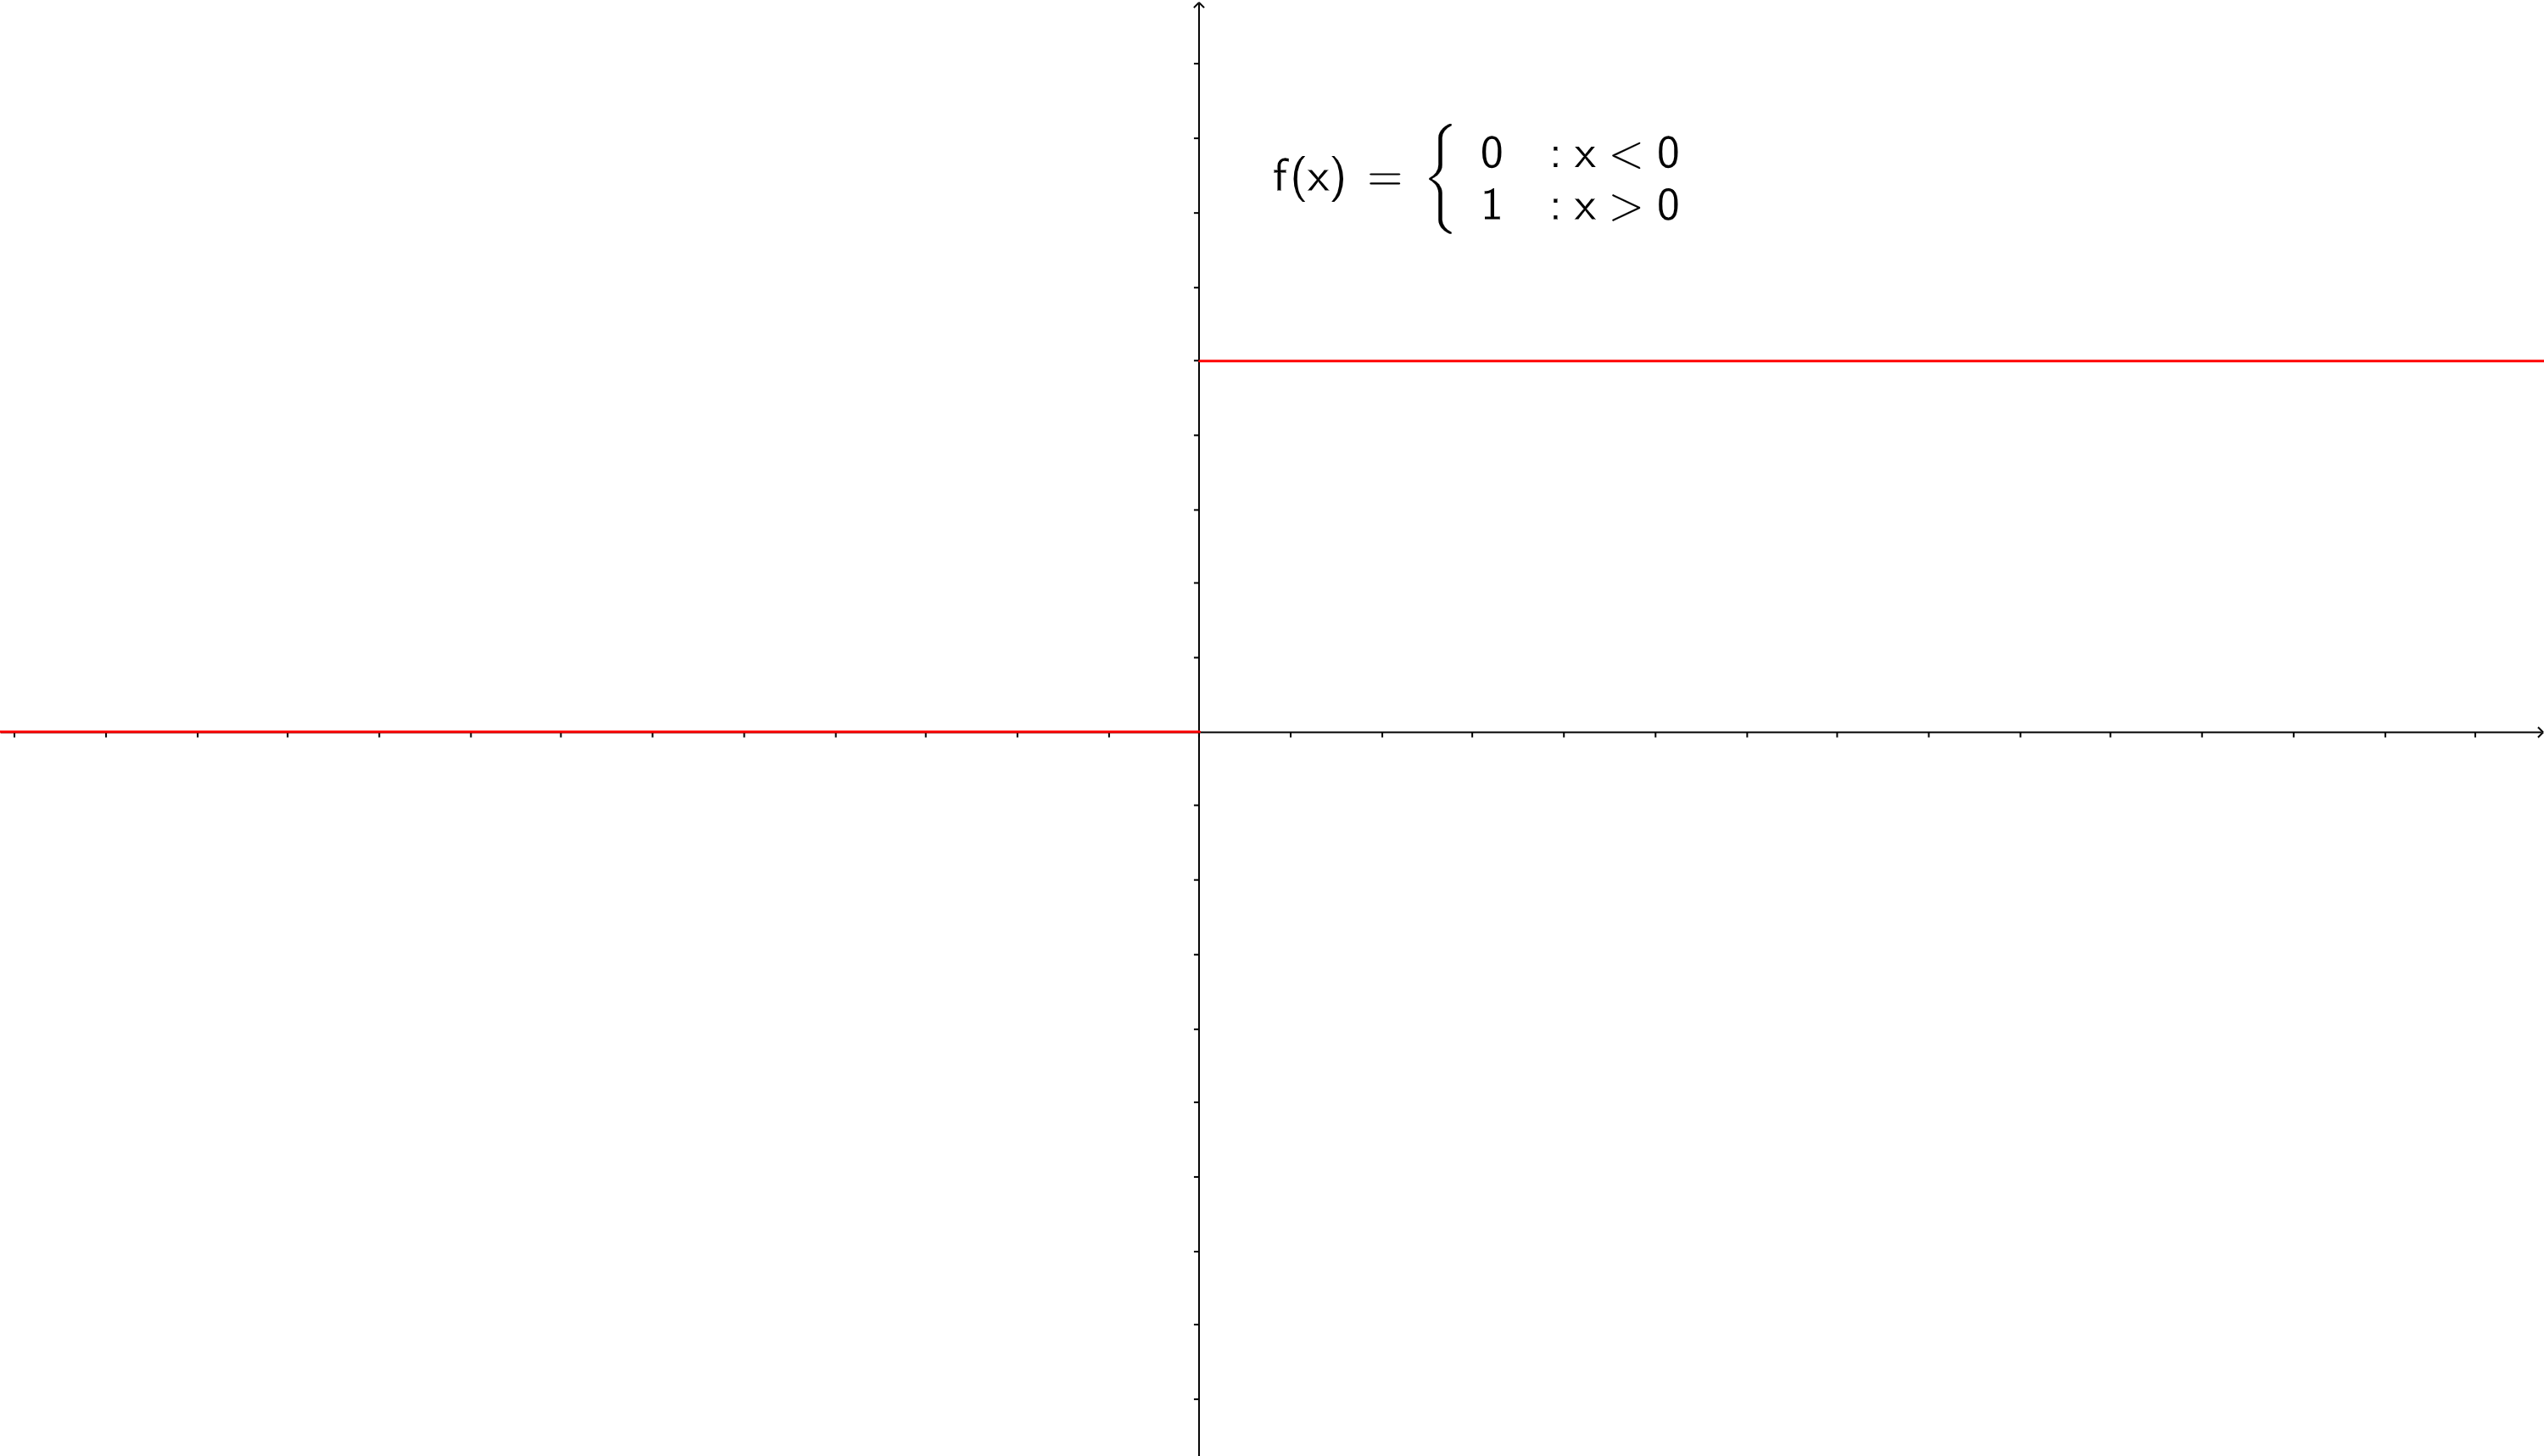
\includegraphics[width=0.5\textwidth,alt={A plot of a step function.}]{figures/step_function}
  %}{A plot of the tan function. }
    \caption{A plot of a step function from \cref{eq: step function} produced using GeoGebra.}
\label{fig: step function}
\end{figure}

\begin{ex}
Consider the step function
\begin{equation}
f(x)=\begin{cases}
&0 \quad x < 0\\
&1 \quad x\geq 0,
\end{cases}
\label{eq: step function}
\end{equation}
shown in \cref{fig: step function}. By looking at the graph we see that the limit of $f(x)$ as $x\to 0$ will depend on the direction of approach. If we start from below zero it is clear that $f(x)\to 0$, while starting above zero it is clear that $f(x)\to 1$. In contrast to the case of $\tan(x)$ the function is not diverging in the limit, but we still end up with a \textbf{One Sided Limit}\footnote{This just means that the function is well behaved in the limit as long as we only look at one side. }
\end{ex} 



\begin{mdiv}
Note that it can be dangerous to use $\infty$ in calculations as if it were a number. This is because there are certain limits and other expressions that we may see which do not make sense:
\begin{equation*}
\infty^{0}, \quad \infty-\infty, \quad \frac{0}{0}, \quad 0^{0}, \quad \frac{\infty}{\infty}, \quad \frac{\infty}{0}, \quad \frac{1}{0}.
\end{equation*}
Just because we see one of these expressions coming out a limit does not necessarily mean that the limit does not exist. It can instead mean that we need to be very careful how we evaluate the limit. In \cref{sec:advanced topics} we will discuss L'H\^{o}pital's rule which is a techniques for evaluating limits that initially look like they do not make sense.
\end{mdiv}

There are a few limits that we need to know that we will not prove here, time permitting we will prove these in \cref{sec:advanced topics}, but you can also look at the ``Proof of Trig Limits'' section of \cite{calcI} to see one approach to proving them. These limits are
\begin{align}
\lim_{x\to 0}\frac{\sin x}{x}&=1, \label{eq: sin limit}\\
\lim_{x\to 0}\frac{\cos x -1}{x}&=0, \label{eq: cos limit}\\
\lim_{h\to 0}\frac{e^{h}-1}{h}&=1, \label{eq: exp limit}\\
\lim_{h\to 0}\frac{\ln(1+h)}{h}&=1. \label{eq: ln limit}
\end{align}
Note that \cref{eq: exp limit} is equivalent to \cref{eq: exp approximation} which we discussed above as one of the definitions of the exponential function.

\section{Continuity and differentiability}
\label{sec: continuity}
Now that we have some examples of functions and understand how to take limits, we can define two properties of a function which will be very important later in the course: \textbf{continuity} and \textbf{differentiability}. \\

A function $f(x)$ is said to be continuous at a point $x=a$ if
\begin{equation}
\lim_{x\to a}f(x)=f(a).
\label{eq: continuity}
\end{equation}

If $X$ is the domain of $f(x)$, we say that $f$ is continuous on $X$ if it is continuous at each point in $X$, often we would just say that $f$ is a continuous function. As a rule of thumb, we can say that a function is continuous if its graph can be drawn from start to finish without taking your pen off the paper. Functions which are not continuous will have jumps or divergences at the point that fails to be continuous.\\

If we have a rational function then we can find where it is not continuous, called being \textbf{discontinuous}, by finding the roots of the denominator.\\

\begin{mdiv}
If we are being careful we need to give three parts to the definition of continuity: 
\begin{itemize}
%\setlength{\itemsep}{-5pt}
    \item[1)] The limit of $f(x)$ as $x\to a$ exists.
    \item[2)] The value of $f(x)$ is defined at $x=a$. i.e. $f(a)$ is defined and is finite.
   \item[3)] The limit of $f(x)$ as $x\to a$ agrees with the value of $f(a)$.
\end{itemize}
This is another place where as this is not a course for mathematicians we can combine all three of these into the one statement in \cref{eq: continuity}. This is another example of being able to use a working definition and not needing to get sidetracked by all of the technical details.
\end{mdiv}

\begin{ex}
We have already met several examples of continuous and discontinuous functions:
\begin{itemize}
%\setlength{\itemsep}{-5pt}
    \item The trig functions $\cos(x)$ and $\sin(x)$ are continuous on all of $\R$.
    \item The exponential function $\exp(x)$ is continuous on all of $\R$.
   \item The natural logarithm is continuous on the positive real numbers $\R$ as, currently we have not defined it for negative $x$, and it diverges in the limit $x\to 0$.
   \item The tangent function $\tan(x)$ are not continuous on $\R$ due to its divergences at $\pm\frac{\uppi}{2},\pm\frac{3\uppi}{2},\dots{}$. However, it is continuous on its domain\footnote{Strictly speaking this is the principle domain of $\tan(x)$ its domain is really $\{x\in \R\vert x\neq \uppi/2 +n\uppi, n\in \Z\}$} $\left(-\frac{\uppi}{2},\frac{\uppi}{2}\right)$
   \item The step function of \cref{eq: step function} is not continuous at $x=0$.
\item The function in \cref{eq: reciprocal of x-2} has a discontinuity at $x=2$
\end{itemize}
\end{ex}
\begin{exercise}
Use the definition of continuity to determine if the function
\begin{equation}
g(x)=\frac{4x+10}{x^{2}-2x-15}
\end{equation}
is continuous and if not find the points where it has discontinuities.
\end{exercise}

Related to continuity is differentiability. A function $f(x)$ is differentiable at a point $a$ if the limit
\begin{equation*}
\lim_{x\to a}\frac{f(x)-f(a)}{x-a}
\end{equation*}
exists. We call this limit the derivative of the function at the point $a$,
\begin{equation}
f'(a)=\lim_{x\to a}\frac{f(x)-f(a)}{x-a},
\label{eq: rate of change at a}
\end{equation}
the notation $\frac{\ud f}{\ud x}(a)$ is sometimes used instead of $f'(a)$. A function is called continuously differentiable if its derivative is also continuous.\\

It is important to note that differentiability at $a$ implies continuity at $a$, but continuity does not imply differentiability.  For example the absolute value function shown in \cref{fig: abs function} is continuous everywhere, but is only differentiable everywhere except at $x=0$.

\begin{figure}[htbp]
    \centering
\ThisAltText{Graph of the absolute value function.}
%    \pdftooltip{
    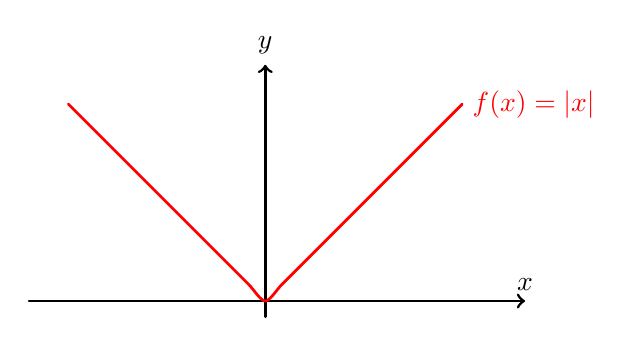
\begin{tikzpicture}[line width=1pt,line cap=round,line join=round,domain=-2.5:2.5, smooth,variable=\x]
     \draw[->] (-3,0) -- (3.3,0) node[above] {$x$};
  \draw[->] (0,-0.2) -- (0,3) node[above] {$y$};
 \draw[color=red]   plot (\x,{abs(\x)}) node[right] {$f(x)=\vert x\vert$};
    \end{tikzpicture}
%    }{absolute value function}
    \caption{The absolute value function $f(x)=\vert x\vert$ is continuous at every point, but it is not differentiable at the point $x=0$.}
        \label{fig: abs function}
\end{figure}

\begin{ex}
Consider the modulus or absolute value function shown in \cref{fig: abs function}. We have said that this is a continuous function which is not differentiable at $x=0$, but how do we show this? We do it by checking all of the limits.\\

Checking continuity at $x=0$ is left as an exercise. For differentiability we need to check the limits as $x\to 0^{+}$ and $x\to 0^{-}$. 

In the first one we have:
\begin{equation*}
\lim_{x\to 0^{+}}\frac{f(x)-f(0)}{x}=\lim_{x\to 0^{+}}\frac{x-0}{x}\lim_{x\to 0^{+}}1=1,
\end{equation*}
while approaching from the other direction gives:
\begin{equation*}
\lim_{x\to 0^{-}}\frac{f(x)-f(0)}{x}=\lim_{x\to 0^{-}}\frac{(-x)-0}{x}\lim_{x\to 0^{-}}-1=-1.
\end{equation*}
These do not agree, so the limit does not exist and the modulus function is not differentiable.
\end{ex}

\begin{figure}[ht]
    \centering
    %\pdftooltip{
\ThisAltText{Graph of a straight line function.}
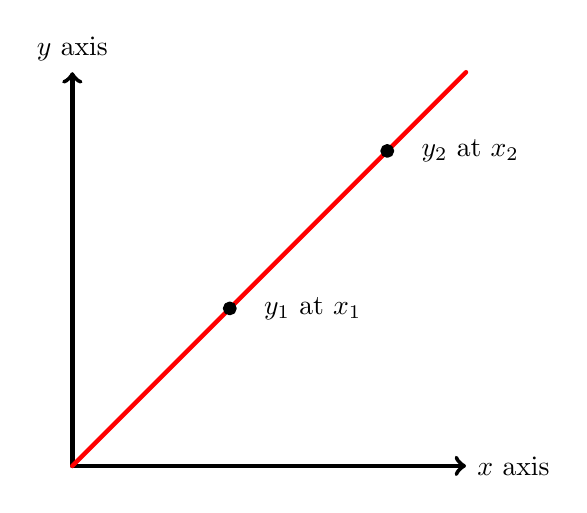
\begin{tikzpicture}[line width=1pt,line cap=round,line join=round]
\draw[black, ultra thick,->] (0,0) --(5,0) node[anchor=west]{$x$ axis};
\draw[black, ultra thick,->] (0,0) --(0,5) node[anchor=south]{$y$ axis};
%\draw[step=1cm,gray,very thin] (-2,-2) grid (6,6);
%\draw[blue, ultra thick] (0,0) parabola (6,6);
\draw[red, ultra thick] (0,0) -- (5,5);
 \filldraw[black] (2,2) circle (2pt) node[right,xshift=3mm]{$y_{1}$ at $x_{1}$};
 \filldraw[black] (4,4) circle (2pt) node[right,xshift=3mm]{$y_{2}$ at $x_{2}$};
\end{tikzpicture}
%}{A displacement time graph showing the difference between constant velocity motion and motion with a changing velocity.}
    \caption{A plot of the straight line $y=x$ and example of $y=mx+c$ with gradient $m=1$ and $y$-intercept $c=0$, with two points on the line marked.}
    \label{fig: straight line graph.}
\end{figure}

The fraction in \cref{eq: rate of change at a} may look familiar to you. If we had a straight line $y=f(x)=mx+c$ where $m$ is the gradient of the straight line and $c$ is the $y$-intercept, then calculating this fraction gives
\begin{equation*}
\frac{f(x)-f(a)}{x-a}=\frac{mx+c-(ma+c)}{x-a}=\frac{m(x-a)}{x-a}=m,
\end{equation*}
which is the gradient of the curve. For a function that is not a straight line, this procedure gives the gradient of the straight line between $x$ and $a$. In the limit that $x\to a$ this fraction becomes the gradient of the \textbf{tangent} line\footnote{A tangent is a line that touches a curve at one point} to the curve at $a$.   See \cref{fig: parabola tangent} for the example of the tangent to parabola $y=x^{2}$.


\begin{mdiv}
The fraction
\begin{equation*}
\frac{f(x)-f(a)}{x-a}
\end{equation*}
is sometimes referred to as the Newton quotient of the function $f(x)$ at the point $a$. This is after Isaac Newton because when calculating a derivative we are calculating this quotient for smaller and smaller differences $x-a$.
\end{mdiv}

\begin{figure}[ht]
    \centering
\ThisAltText{Graph of a parabola with a tangent curve shown .}
\begin{tikzpicture}[line width=1pt,line cap=round,line join=round]
    \begin{axis}[
            xtick = \empty,    ytick = \empty,
            xlabel = {$x$},
            x label style = {at={(1,0)},anchor=west},
            ylabel = {$y$},
            y label style = {at={(0,1)},rotate=-90,anchor=south},
            axis lines=left,
            enlargelimits=0.2,
        ]
        \addplot[color=black,smooth,thick,-] {(x)^2};
        \addplot[mark=none, red] coordinates {(-6,20) (0,-4)};
    \end{axis}
\end{tikzpicture}
 \caption{A plot of a parabola in black and its tangent in red}
    \label{fig: parabola tangent}
\end{figure}